%
\hsection{Reports}%
\label{sec:factory:reports}%
\FloatBarrier%
%
\begin{figure}%
\centering%
%
\subfloat[][%
We select \menu{Reports} in the \menu{Database} pane and click on \inQuotes{Use Wizard to Create Report\dots}%
\label{fig:factoryLibreOfficeBaseReport01main}%
]{\tightbox{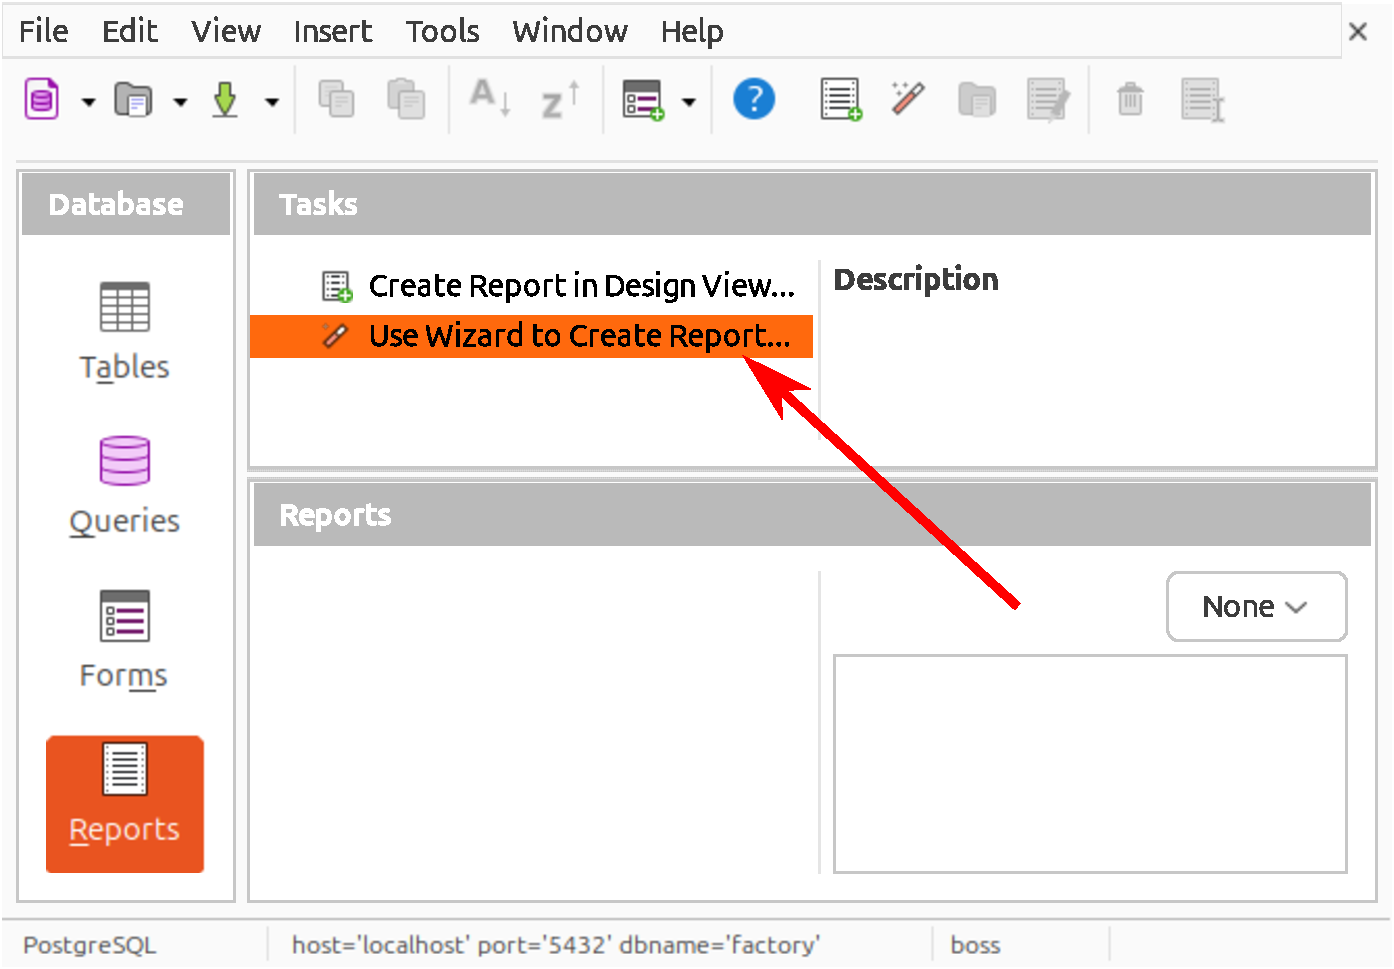
\includegraphics[width=0.49\linewidth]{\currentDir/factoryLibreOfficeBaseReport01main}}}%
%
\floatSep%
%
\subfloat[][%
We need to choose the data source for the new report. %
We click on \inQuotes{Tables \underline{o}r queries.}%
\label{fig:factoryLibreOfficeBaseReport02wizardDataSource}%
]{\tightbox{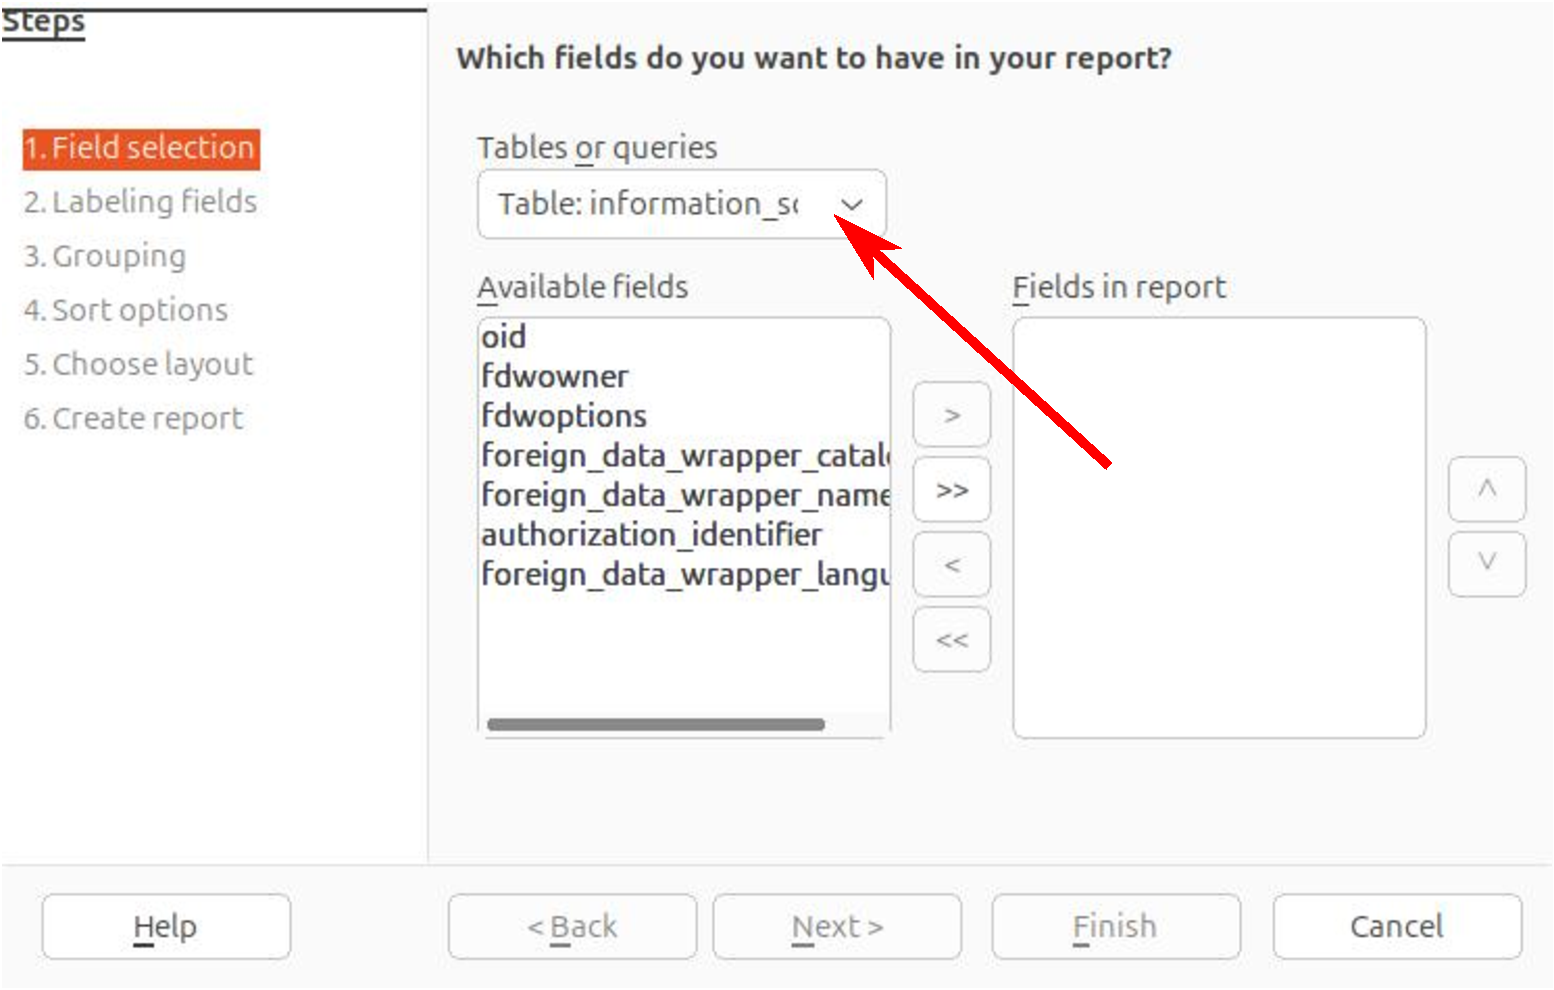
\includegraphics[width=0.49\linewidth]{\currentDir/factoryLibreOfficeBaseReport02wizardDataSource}}}%
%
\floatRowSep%
%
\subfloat[][%
In the table list that pops up, we scroll down all the way an select \inQuotes{Table: public.sale.}%
\label{fig:factoryLibreOfficeBaseReport03wizardDataSource}%
]{\tightbox{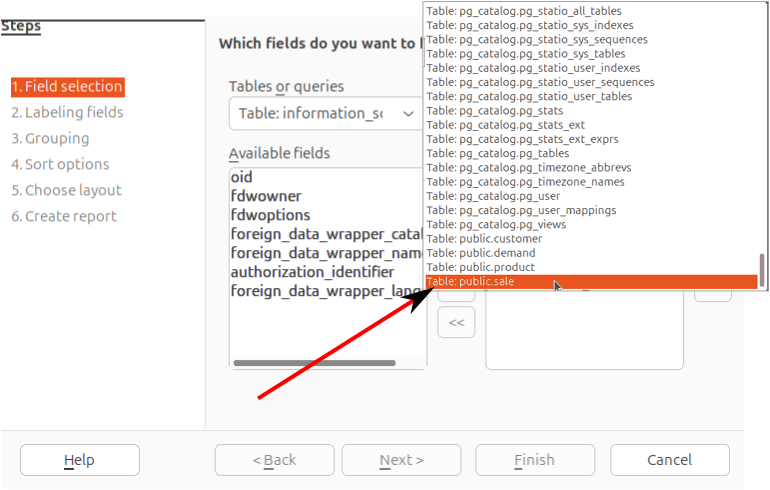
\includegraphics[width=0.49\linewidth]{\currentDir/factoryLibreOfficeBaseReport03wizardDataSource}}}%
%
\floatSep%
%
\subfloat[][%
We get shown all the available columns and select them all. %
Then we click the double wedge \menu{>>} to add them to the \inQuotes{Fields in report} pane.%
\label{fig:factoryLibreOfficeBaseReport04wizardDataFields}%
]{\tightbox{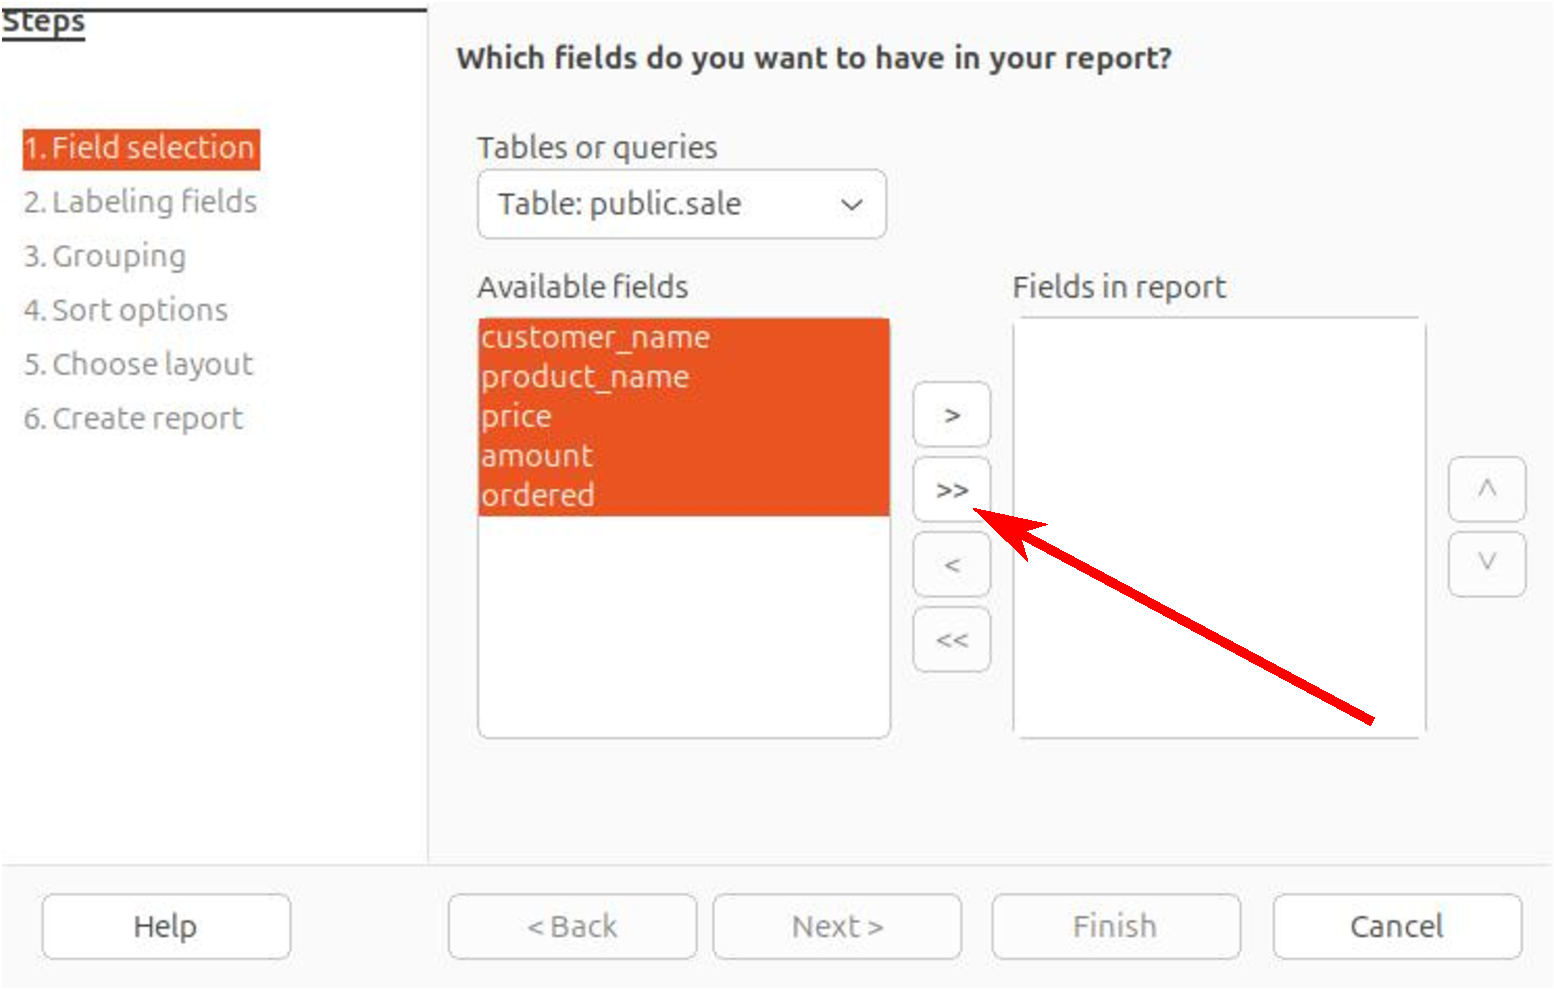
\includegraphics[width=0.49\linewidth]{\currentDir/factoryLibreOfficeBaseReport04wizardDataFields}}}%
%
\floatRowSep%
%
\subfloat[][%
Now that the columns are set up, we click \menu{Next}.%
\label{fig:factoryLibreOfficeBaseReport05wizardDataFieldsChosen}%
]{\tightbox{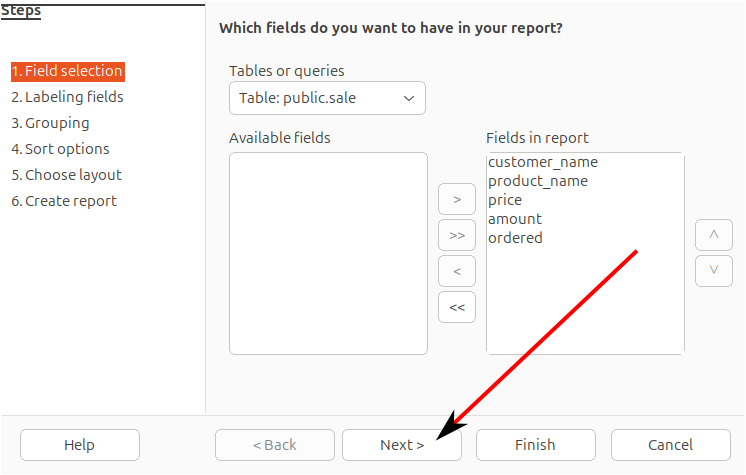
\includegraphics[width=0.49\linewidth]{\currentDir/factoryLibreOfficeBaseReport05wizardDataFieldsChosen}}}%
%
\floatSep%
%
\subfloat[][%
We get asked how we want to label the fields. %
We will enter some more appropriate names.%
\label{fig:factoryLibreOfficeBaseReport06wizardLabels}%
]{\tightbox{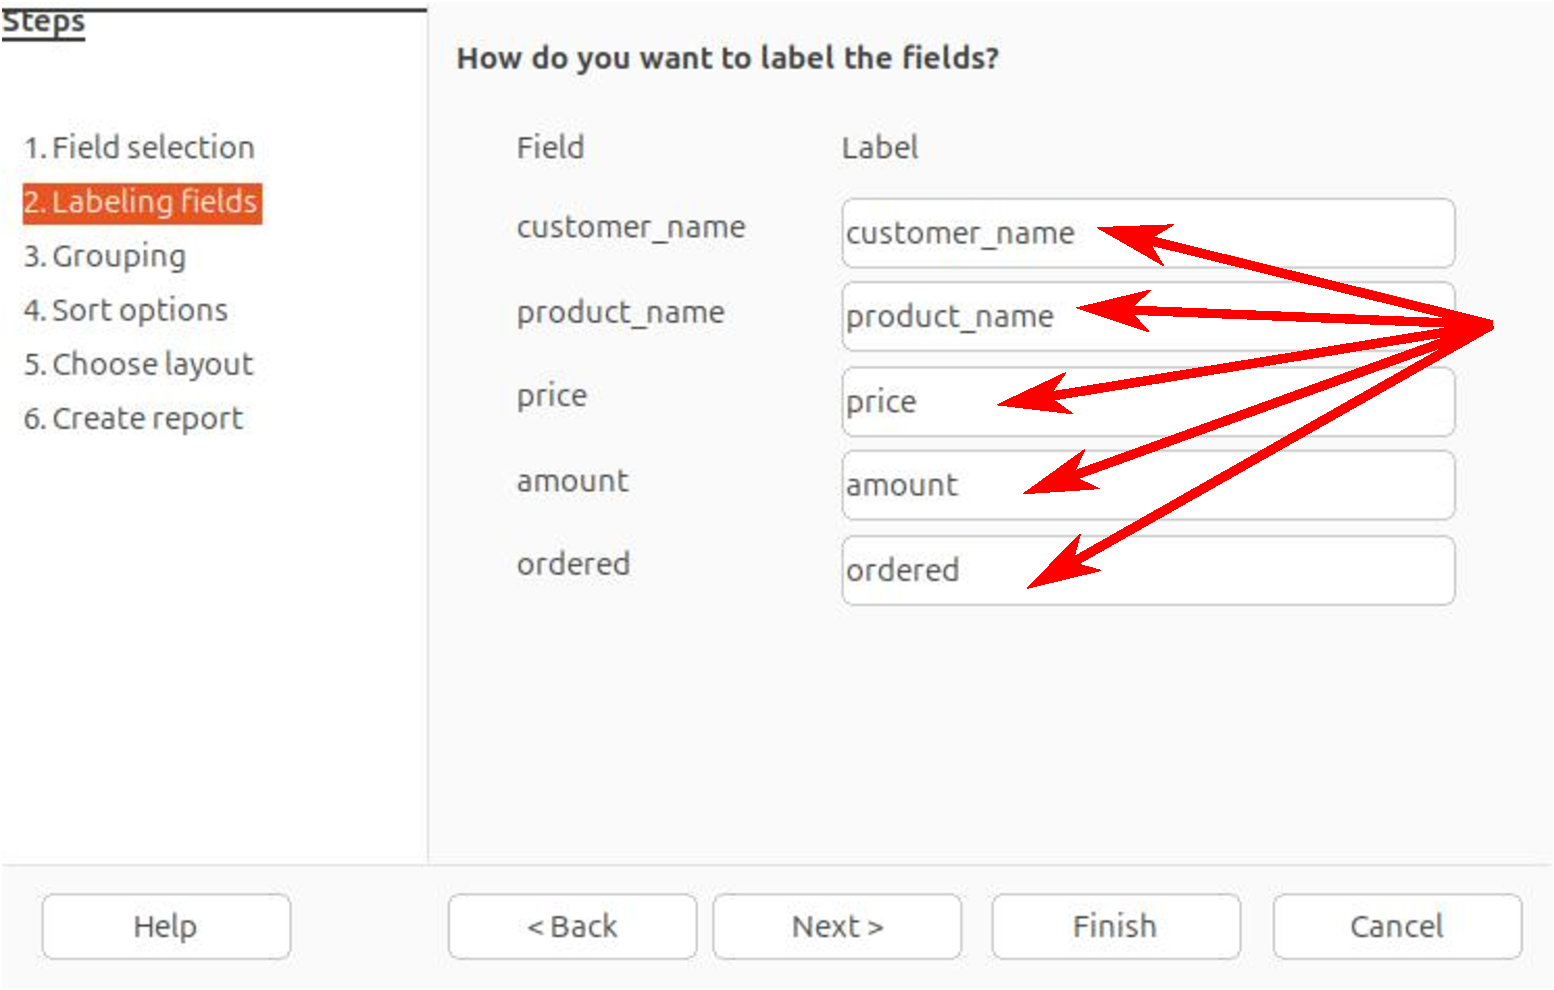
\includegraphics[width=0.49\linewidth]{\currentDir/factoryLibreOfficeBaseReport06wizardLabels}}}%
%
\caption{Creating and executing \db\ reports in \libreofficeBase.}%
\label{fig:factoryLibreOfficeBaseReportA}%
\end{figure}%
%
%
\begin{figure}%
\ContinuedFloat%
\centering%
%
\subfloat[][%
We have chosen more appropriate labels and click \menu{Next}.%
\label{fig:factoryLibreOfficeBaseReport07wizardLabelsChosen}%
]{\tightbox{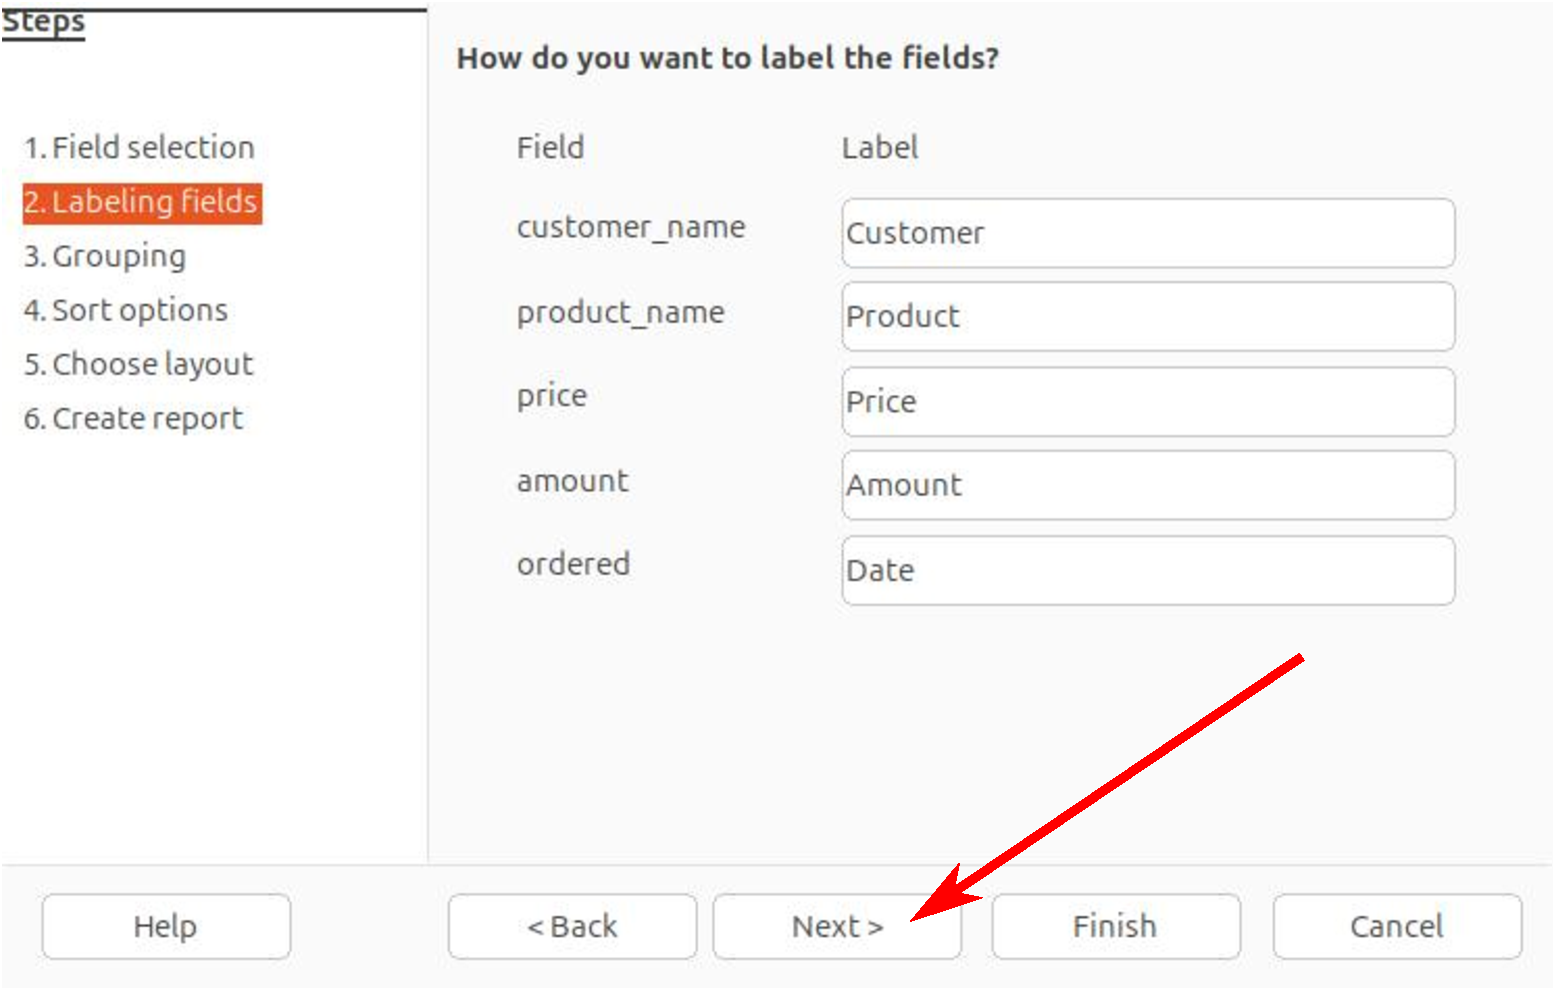
\includegraphics[width=0.49\linewidth]{\currentDir/factoryLibreOfficeBaseReport07wizardLabelsChosen}}}%
%
\floatSep%
%
\subfloat[][%
We now can divide the data into groups. %
We want to divide it into one section per customer in \menu{Fields}. %
So we select \sqlil{customer_name} and click the wedge \menu{>} button to move it to \menu{Groupings}.%
\label{fig:factoryLibreOfficeBaseReport08wizardGrouping}%
]{\tightbox{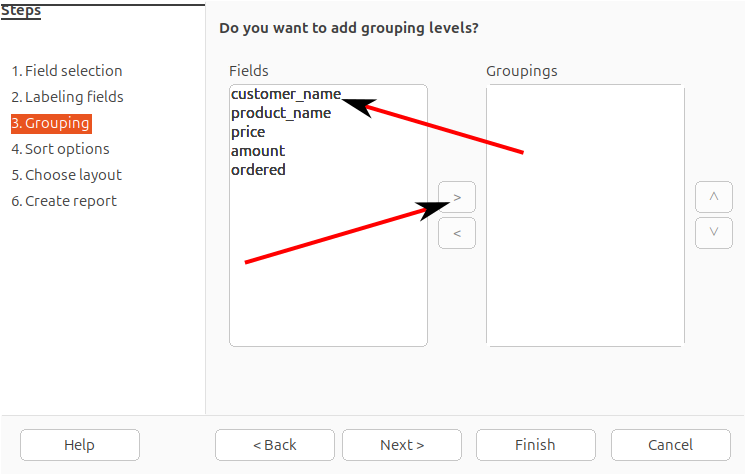
\includegraphics[width=0.49\linewidth]{\currentDir/factoryLibreOfficeBaseReport08wizardGrouping}}}%
%
\floatRowSep%
%
\subfloat[][%
It appears in \menu{Groupings}. %
We click \menu{Next}.%
\label{fig:factoryLibreOfficeBaseReport09wizardGroupingByCustomer}%
]{\tightbox{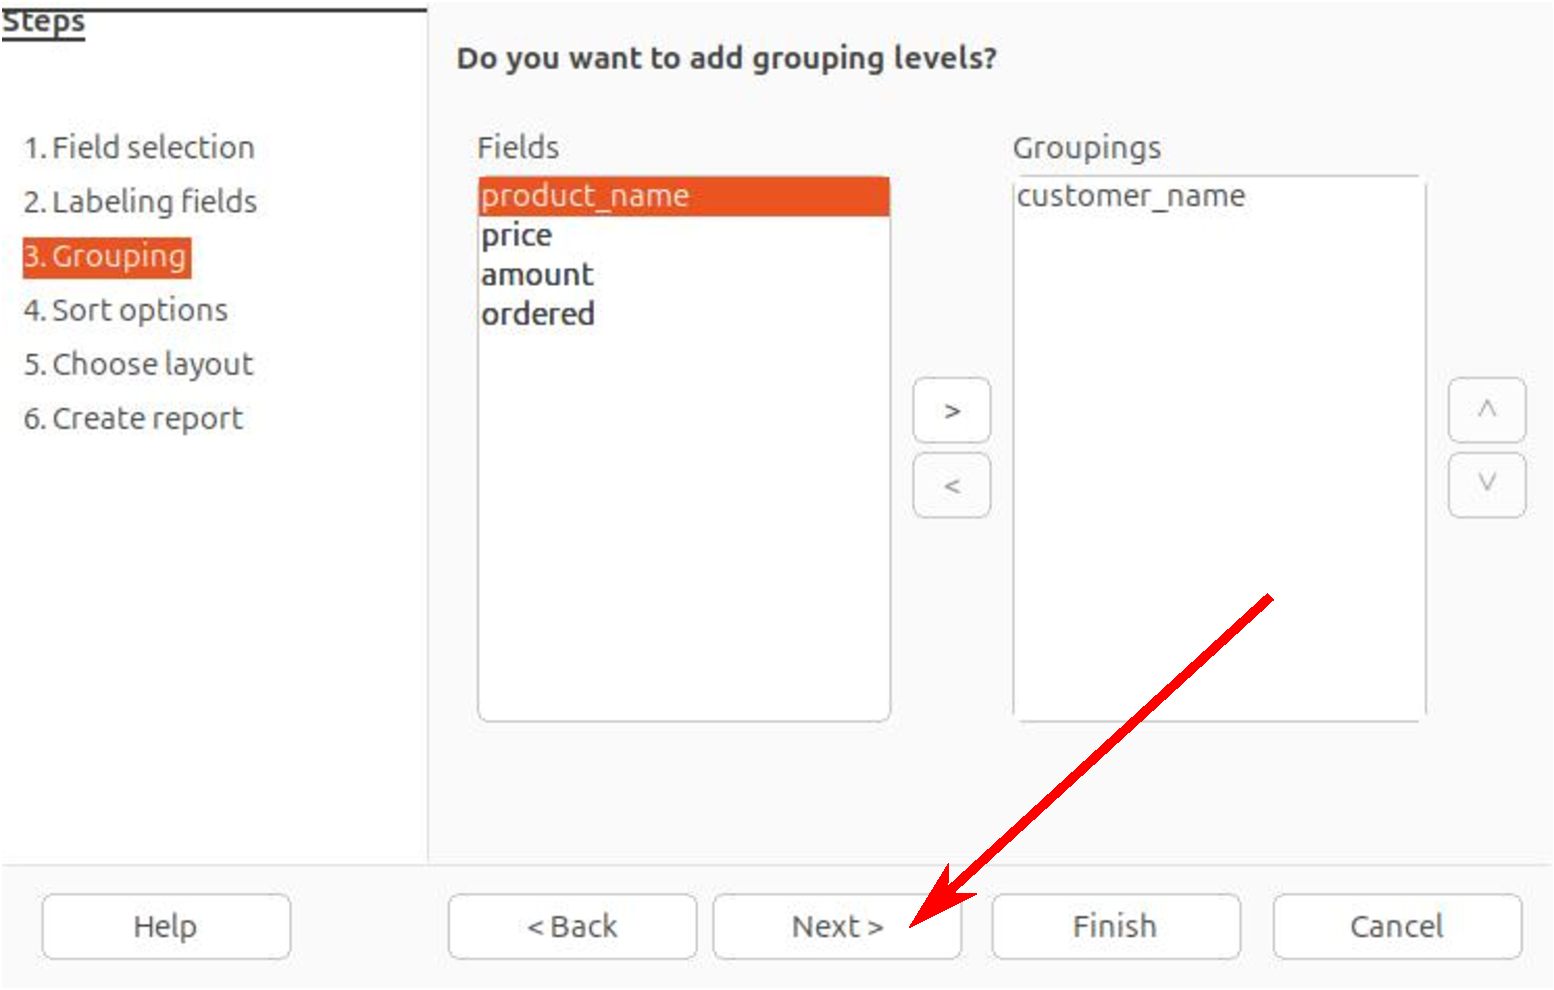
\includegraphics[width=0.49\linewidth]{\currentDir/factoryLibreOfficeBaseReport09wizardGroupingByCustomer}}}%
%
\floatSep%
%
\subfloat[][%
Now we can sort the data. %
It will be sorted by customer, but inside the customer sections, we want to order the sales demands by date, product (in case of tied dates), and amount.%
\label{fig:factoryLibreOfficeBaseReport10wizardSorting}%
]{\tightbox{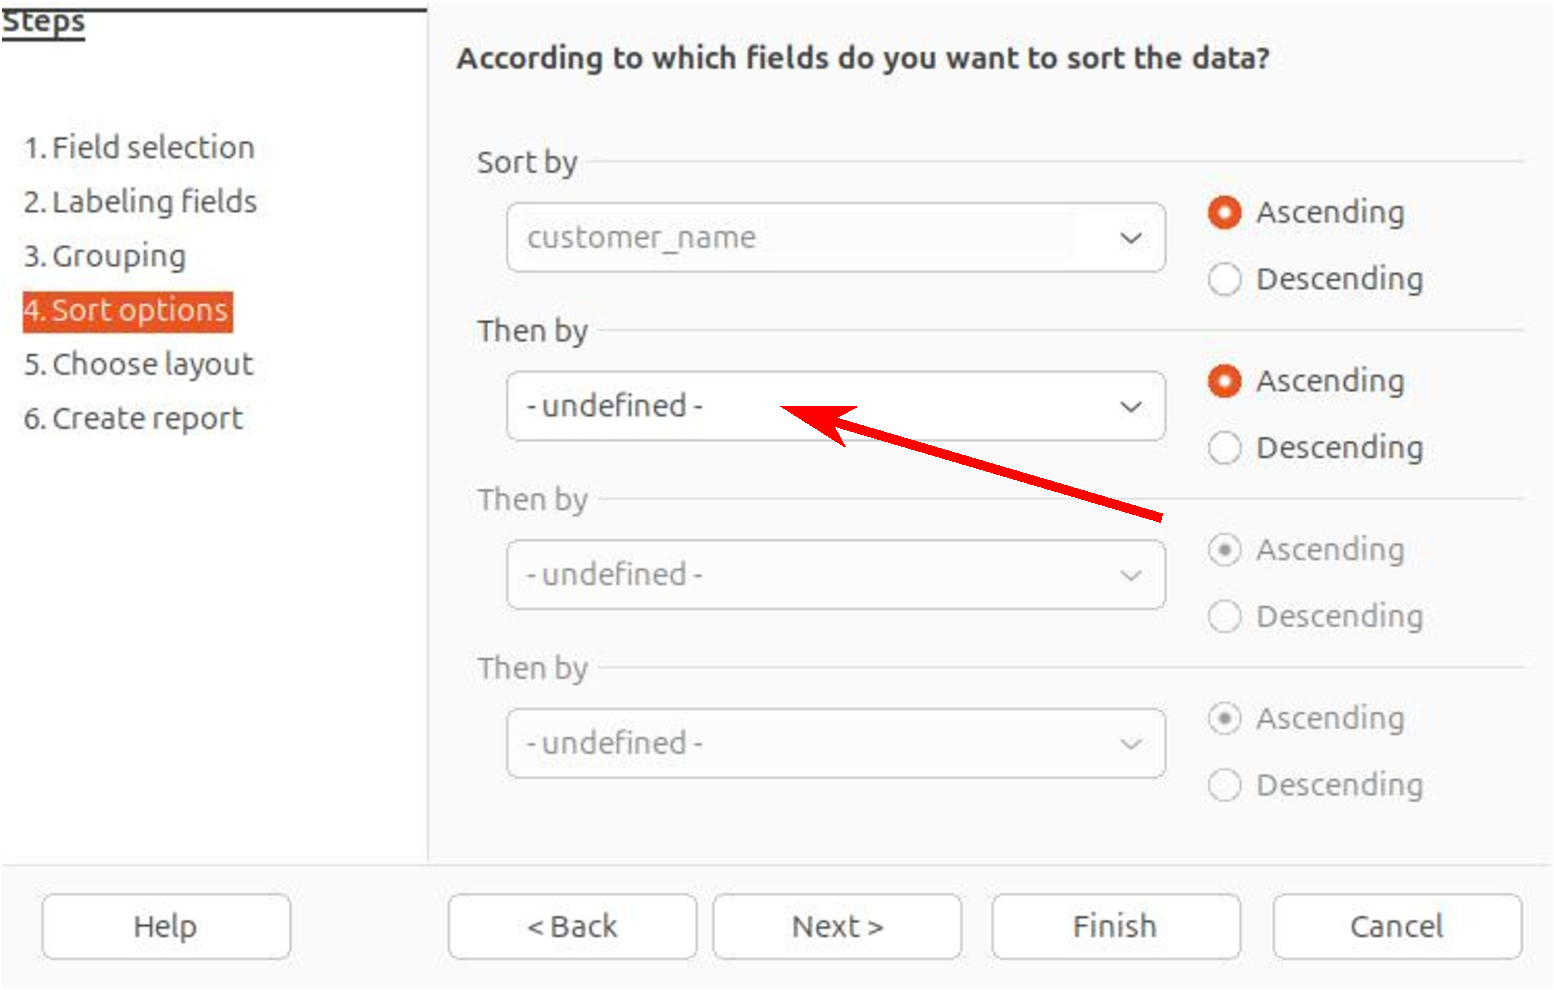
\includegraphics[width=0.49\linewidth]{\currentDir/factoryLibreOfficeBaseReport10wizardSorting}}}%
%
\floatRowSep%
%
\subfloat[][%
We have added the fields. %
(Ordering in descending fashion means bigger values first, ordering in ascending fashion means smaller values first.) %
We click \menu{Next}.%
\label{fig:factoryLibreOfficeBaseReport11wizardSortingFields}%
]{\tightbox{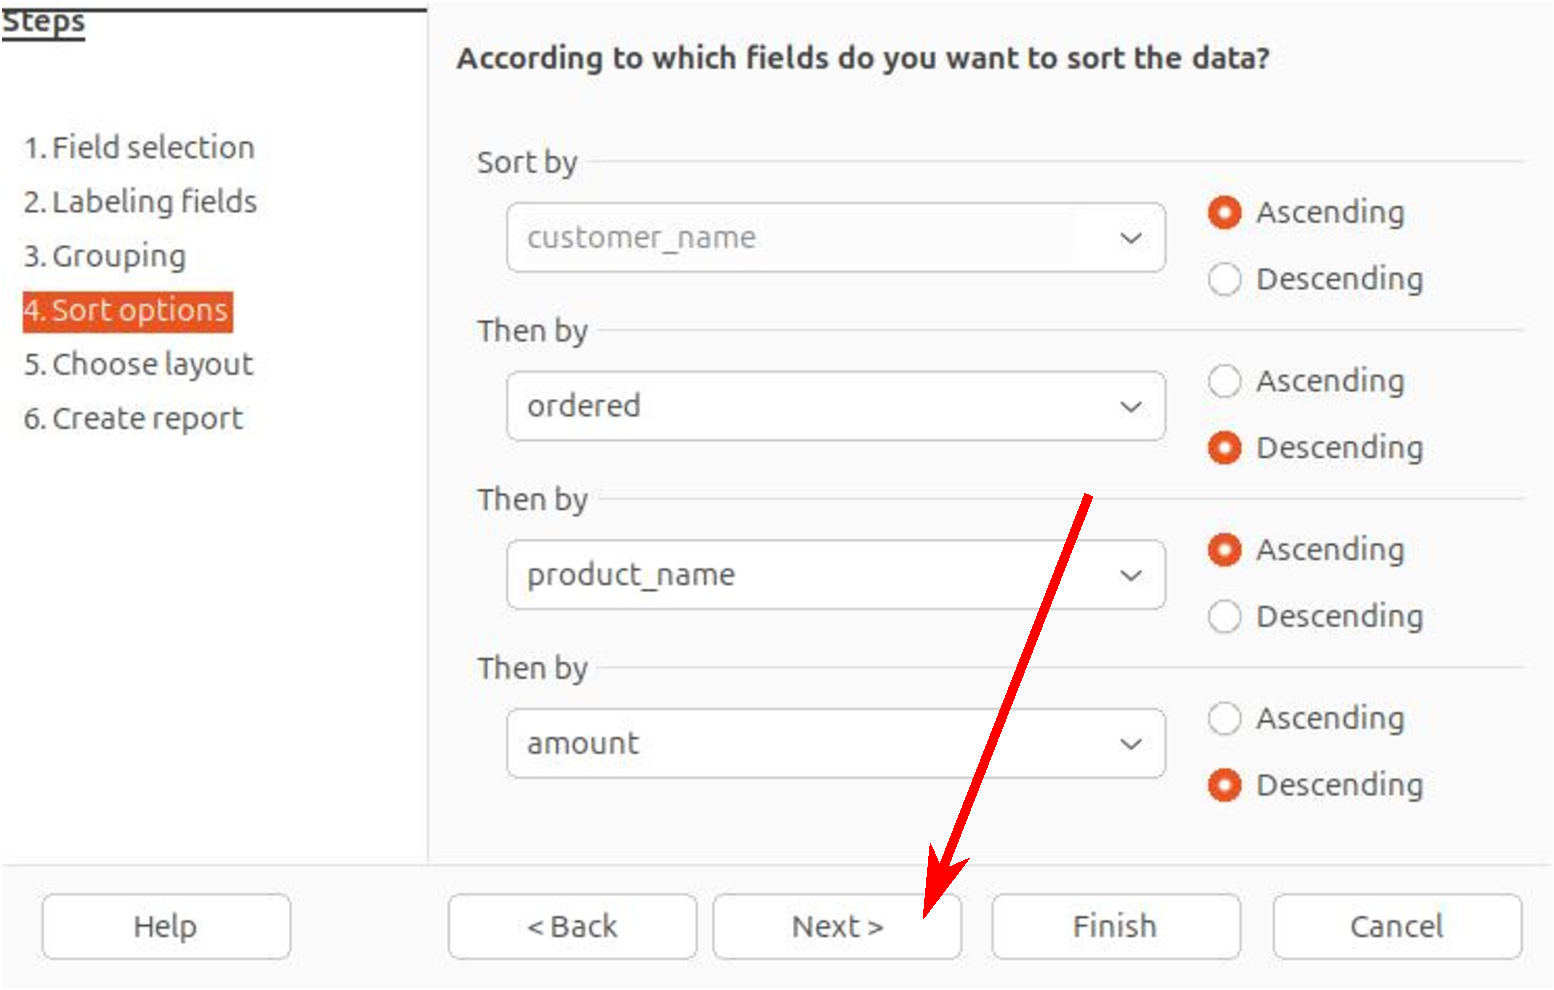
\includegraphics[width=0.49\linewidth]{\currentDir/factoryLibreOfficeBaseReport11wizardSortingFields}}}%
%
\floatSep%
%
\subfloat[][%
We can now choose the layout. %
We are OK with the standard tabular look, but want the report be in portrait format.%
\label{fig:factoryLibreOfficeBaseReport12wizardLayout}%
]{\tightbox{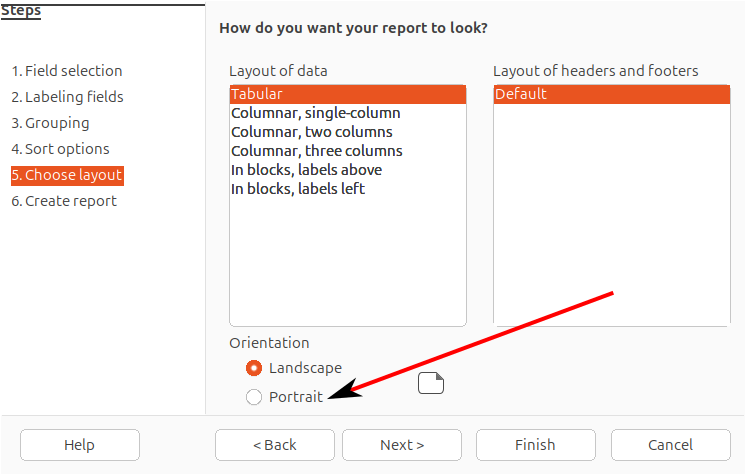
\includegraphics[width=0.49\linewidth]{\currentDir/factoryLibreOfficeBaseReport12wizardLayout}}}%
%
\caption{Creating and executing \db\ reports in \libreofficeBase\ (Continued).}%
\label{fig:factoryLibreOfficeBaseReportB}%
\end{figure}%
%
%
\begin{figure}%
\ContinuedFloat%
\centering%
%
\subfloat[][%
After changing the layout, we click \menu{Next}.%
\label{fig:factoryLibreOfficeBaseReport13wizardPortrait}%
]{\tightbox{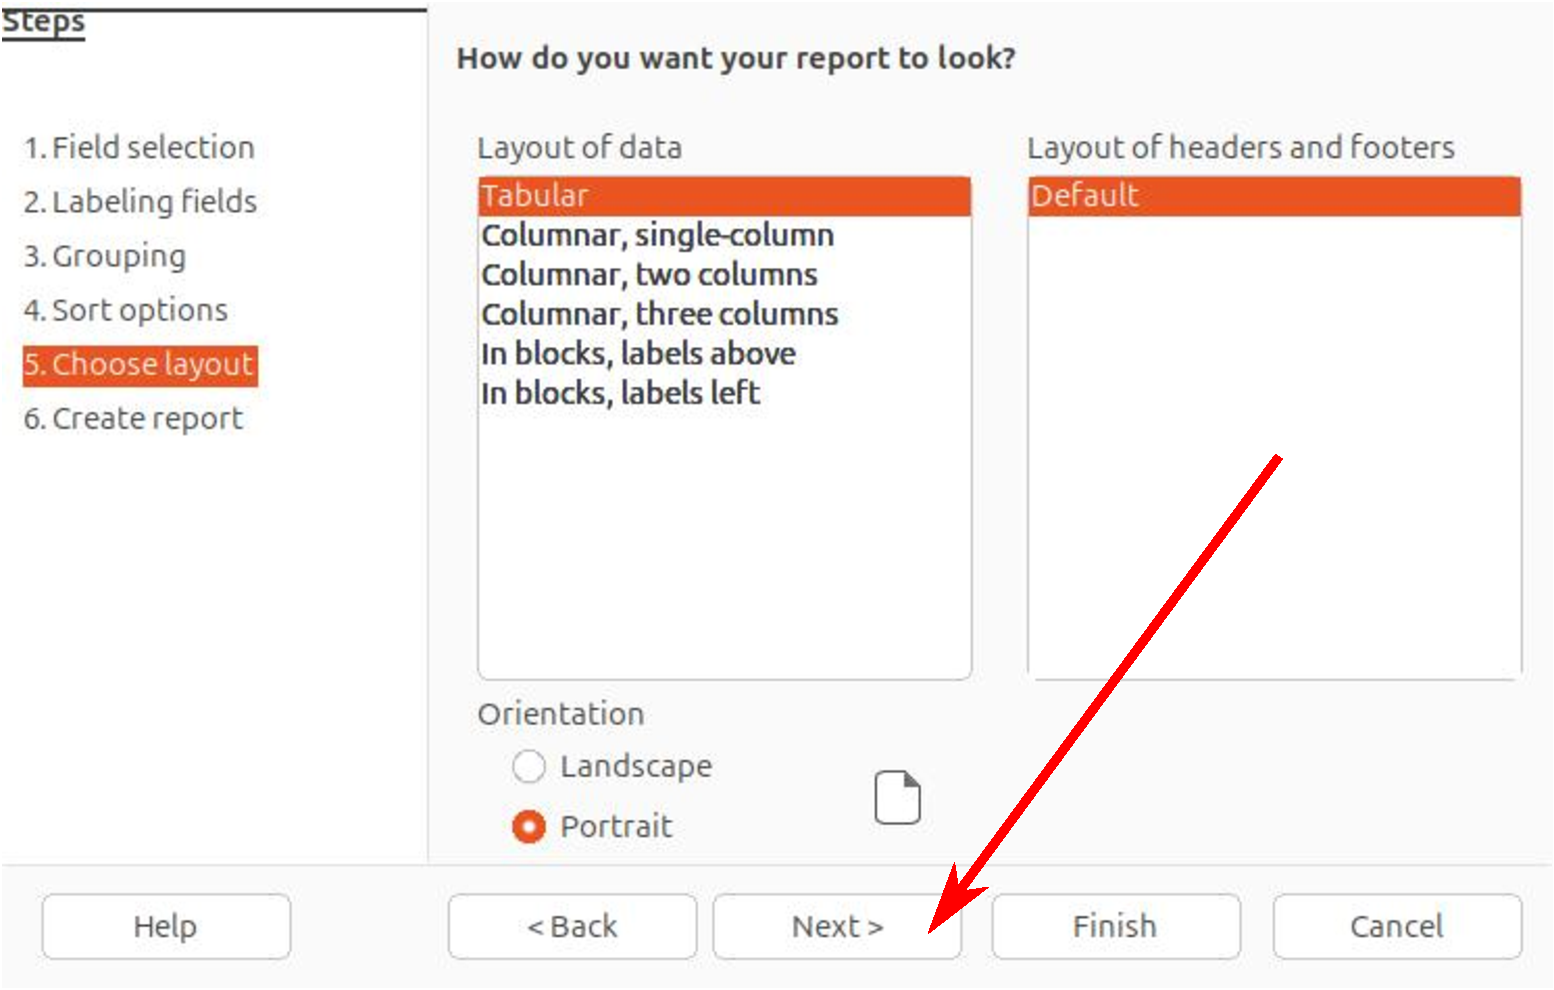
\includegraphics[width=0.49\linewidth]{\currentDir/factoryLibreOfficeBaseReport13wizardPortrait}}}%
%
\floatSep%
%
\subfloat[][%
As report name, we thing \sqlil{sale} will be better than \sqlil{public.sale}.%
\label{fig:factoryLibreOfficeBaseReport14wizardCreate}%
]{\tightbox{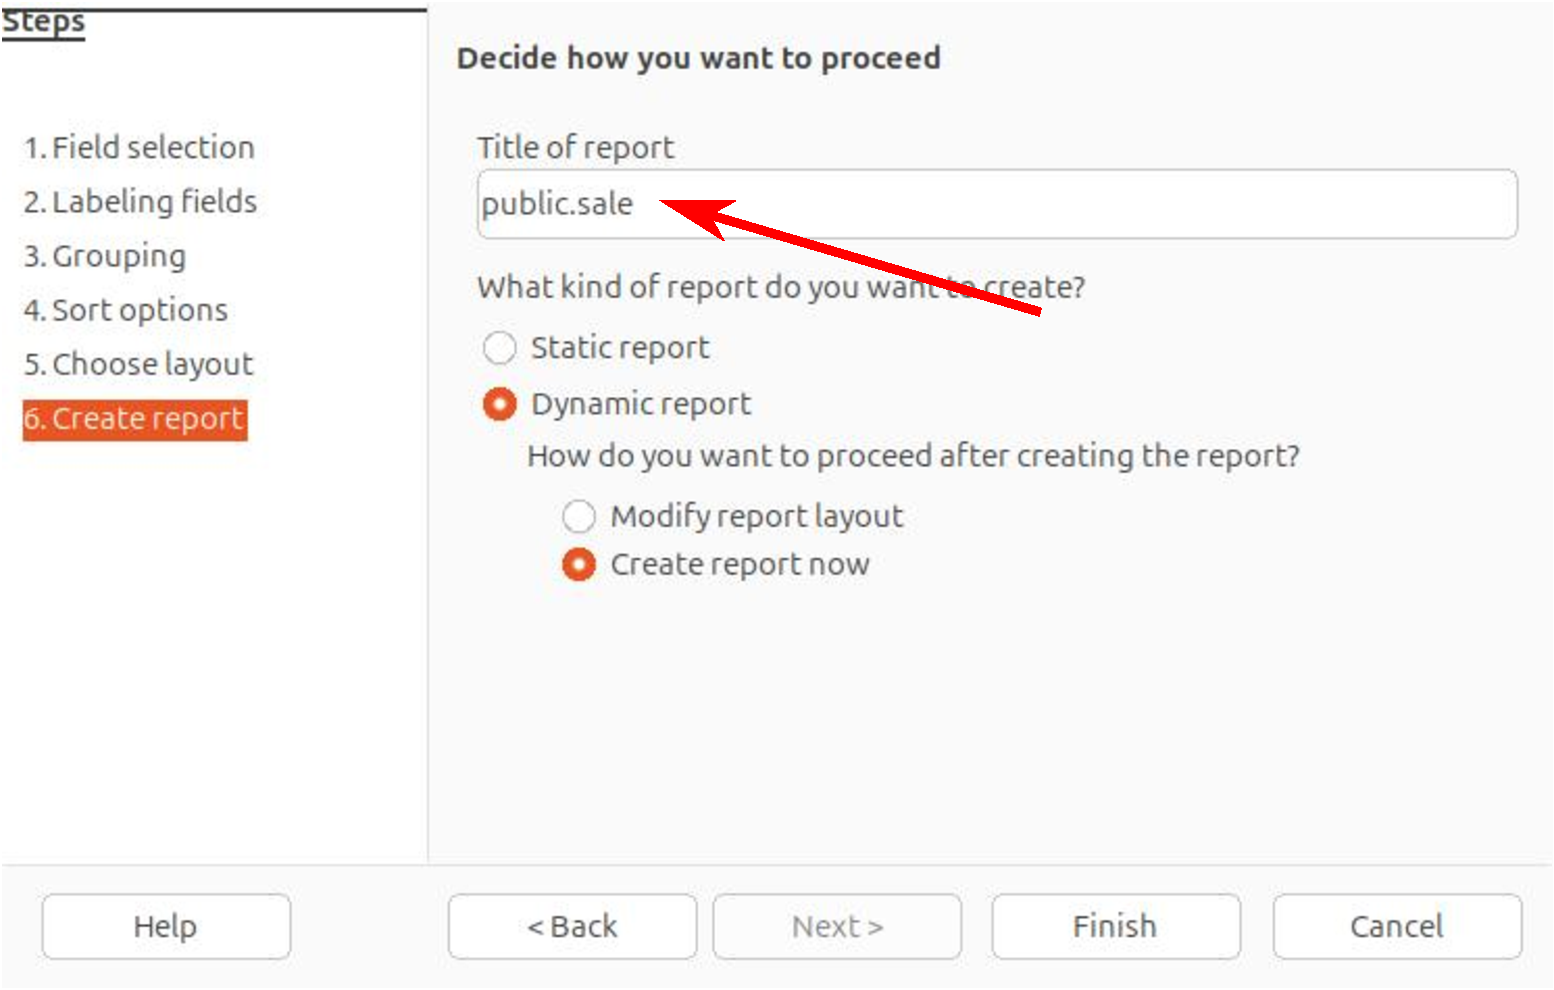
\includegraphics[width=0.49\linewidth]{\currentDir/factoryLibreOfficeBaseReport14wizardCreate}}}%
%
\floatRowSep%
%
\subfloat[][%
We also do not just want to print the report right away, but we want to \inQuotes{Modify report layout.}%
\label{fig:factoryLibreOfficeBaseReport15wizardCreateSale}%
]{\tightbox{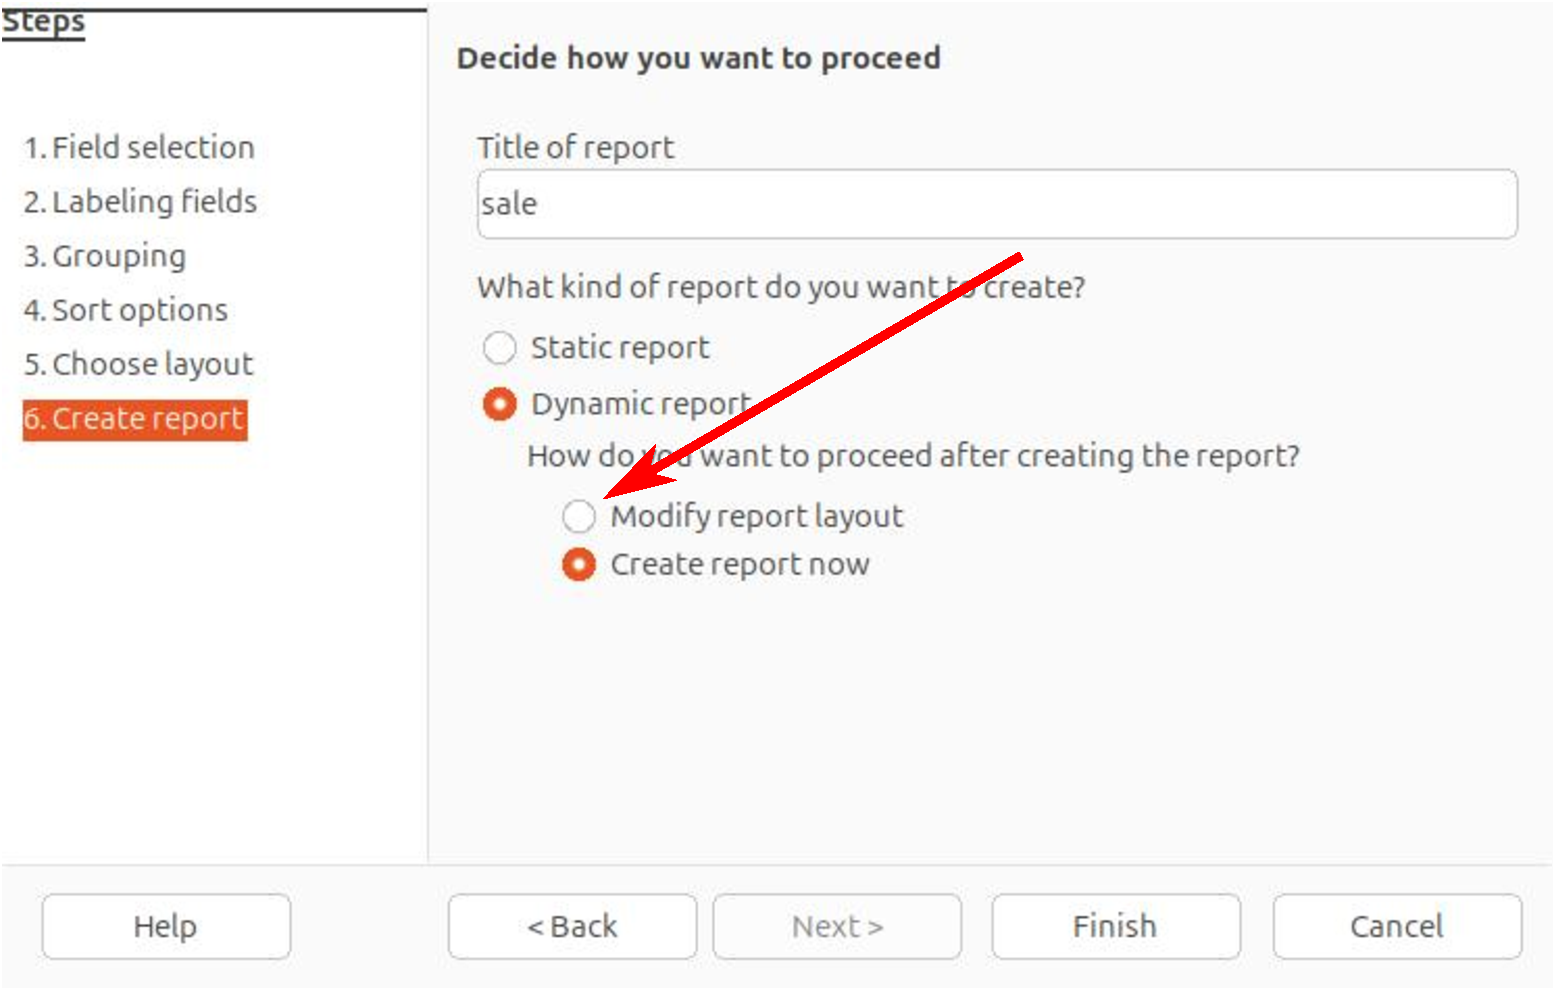
\includegraphics[width=0.49\linewidth]{\currentDir/factoryLibreOfficeBaseReport15wizardCreateSale}}}%
%
\floatSep%
%
\subfloat[][%
We can now click \menu{Next}.%
\label{fig:factoryLibreOfficeBaseReport16wizardCreateModifyLayout}%
]{\tightbox{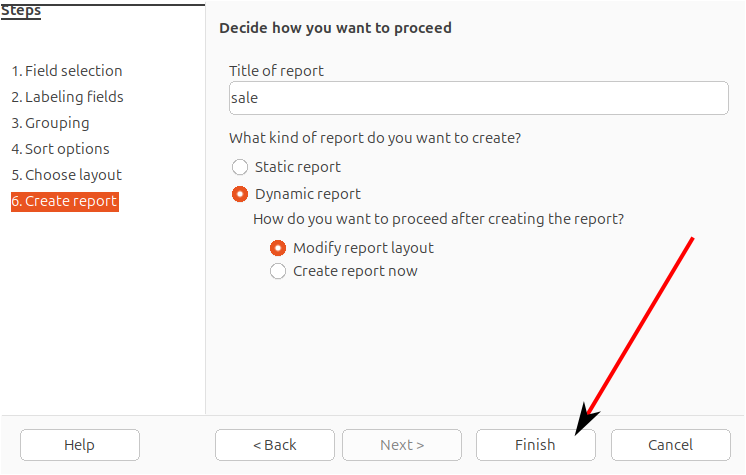
\includegraphics[width=0.49\linewidth]{\currentDir/factoryLibreOfficeBaseReport16wizardCreateModifyLayout}}}%
%
\floatRowSep%
%
\subfloat[][%
The report is create in design view. %
It looks a bit clunky. %
For example, the customer field takes way too much space. %
And it does not need a label. %
So we click the label and pres \keys{\del}.%
\label{fig:factoryLibreOfficeBaseReport17created}%
]{\tightbox{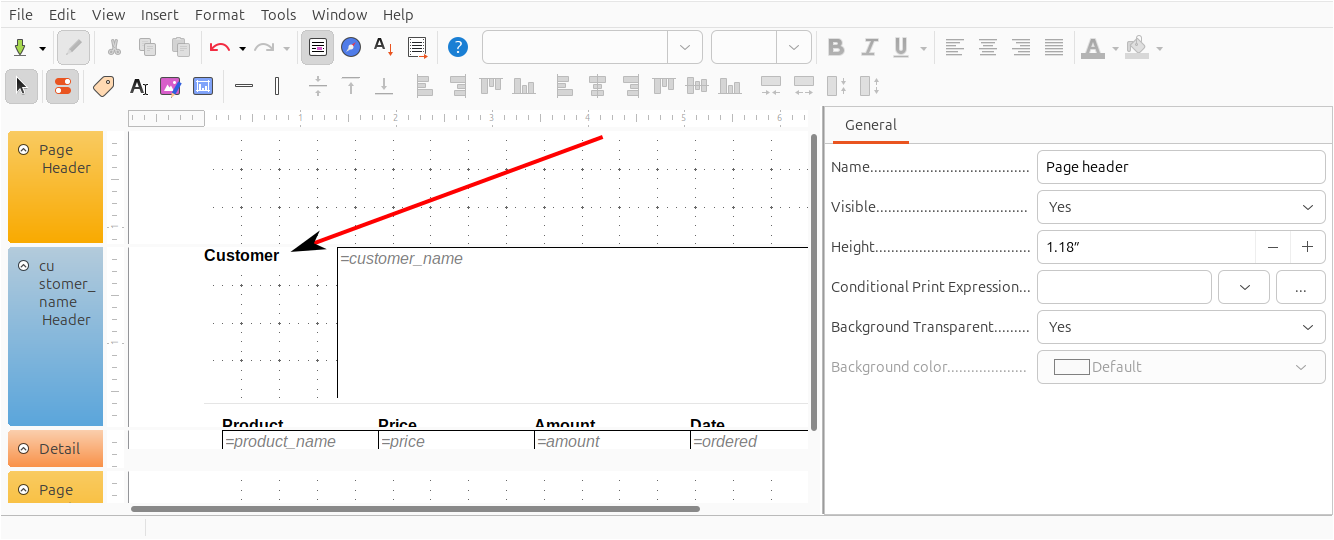
\includegraphics[width=0.49\linewidth]{\currentDir/factoryLibreOfficeBaseReport17created}}}%
%
\floatSep%
%
\subfloat[][%
We also dragged the left corner of the \sqlil{customer} field to the left border. %
We now want to drag its bottom curner up, because it does not need so much space.%
\label{fig:factoryLibreOfficeBaseReport18customerLabelRemoved}%
]{\tightbox{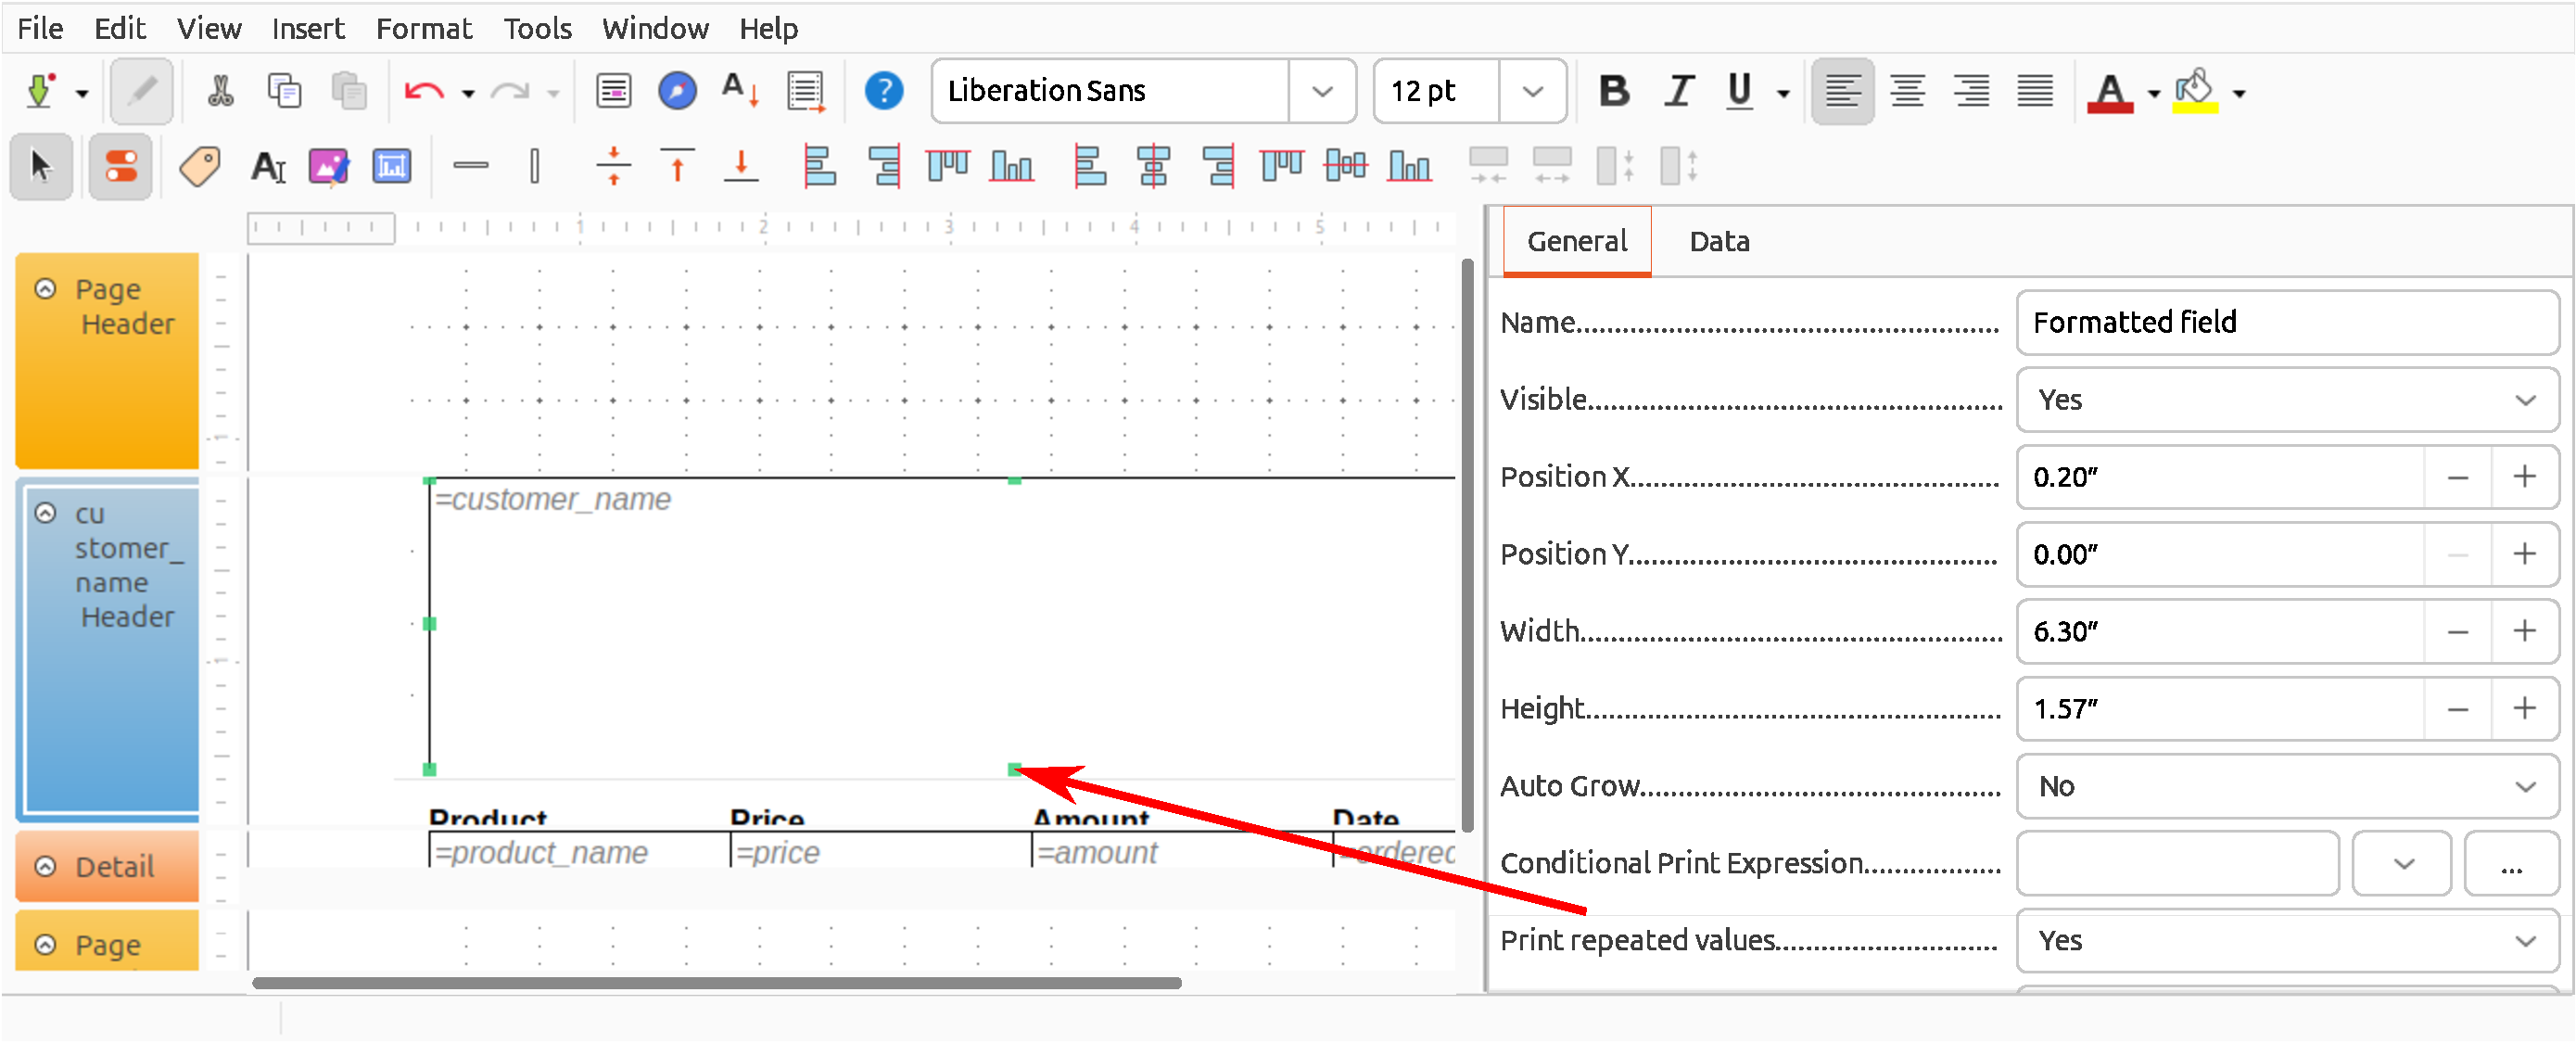
\includegraphics[width=0.49\linewidth]{\currentDir/factoryLibreOfficeBaseReport18customerLabelRemoved}}}%
%
%
\caption{Creating and executing \db\ reports in \libreofficeBase\ (Continued).}%
\label{fig:factoryLibreOfficeBaseReportC}%
\end{figure}%
%
%
\begin{figure}%
\ContinuedFloat%
\centering%
%
\subfloat[][%
Now it has an appropriate size. %
Next we want to move all the table headers upward.%
\label{fig:factoryLibreOfficeBaseReport19customerShrinked}%
]{\tightbox{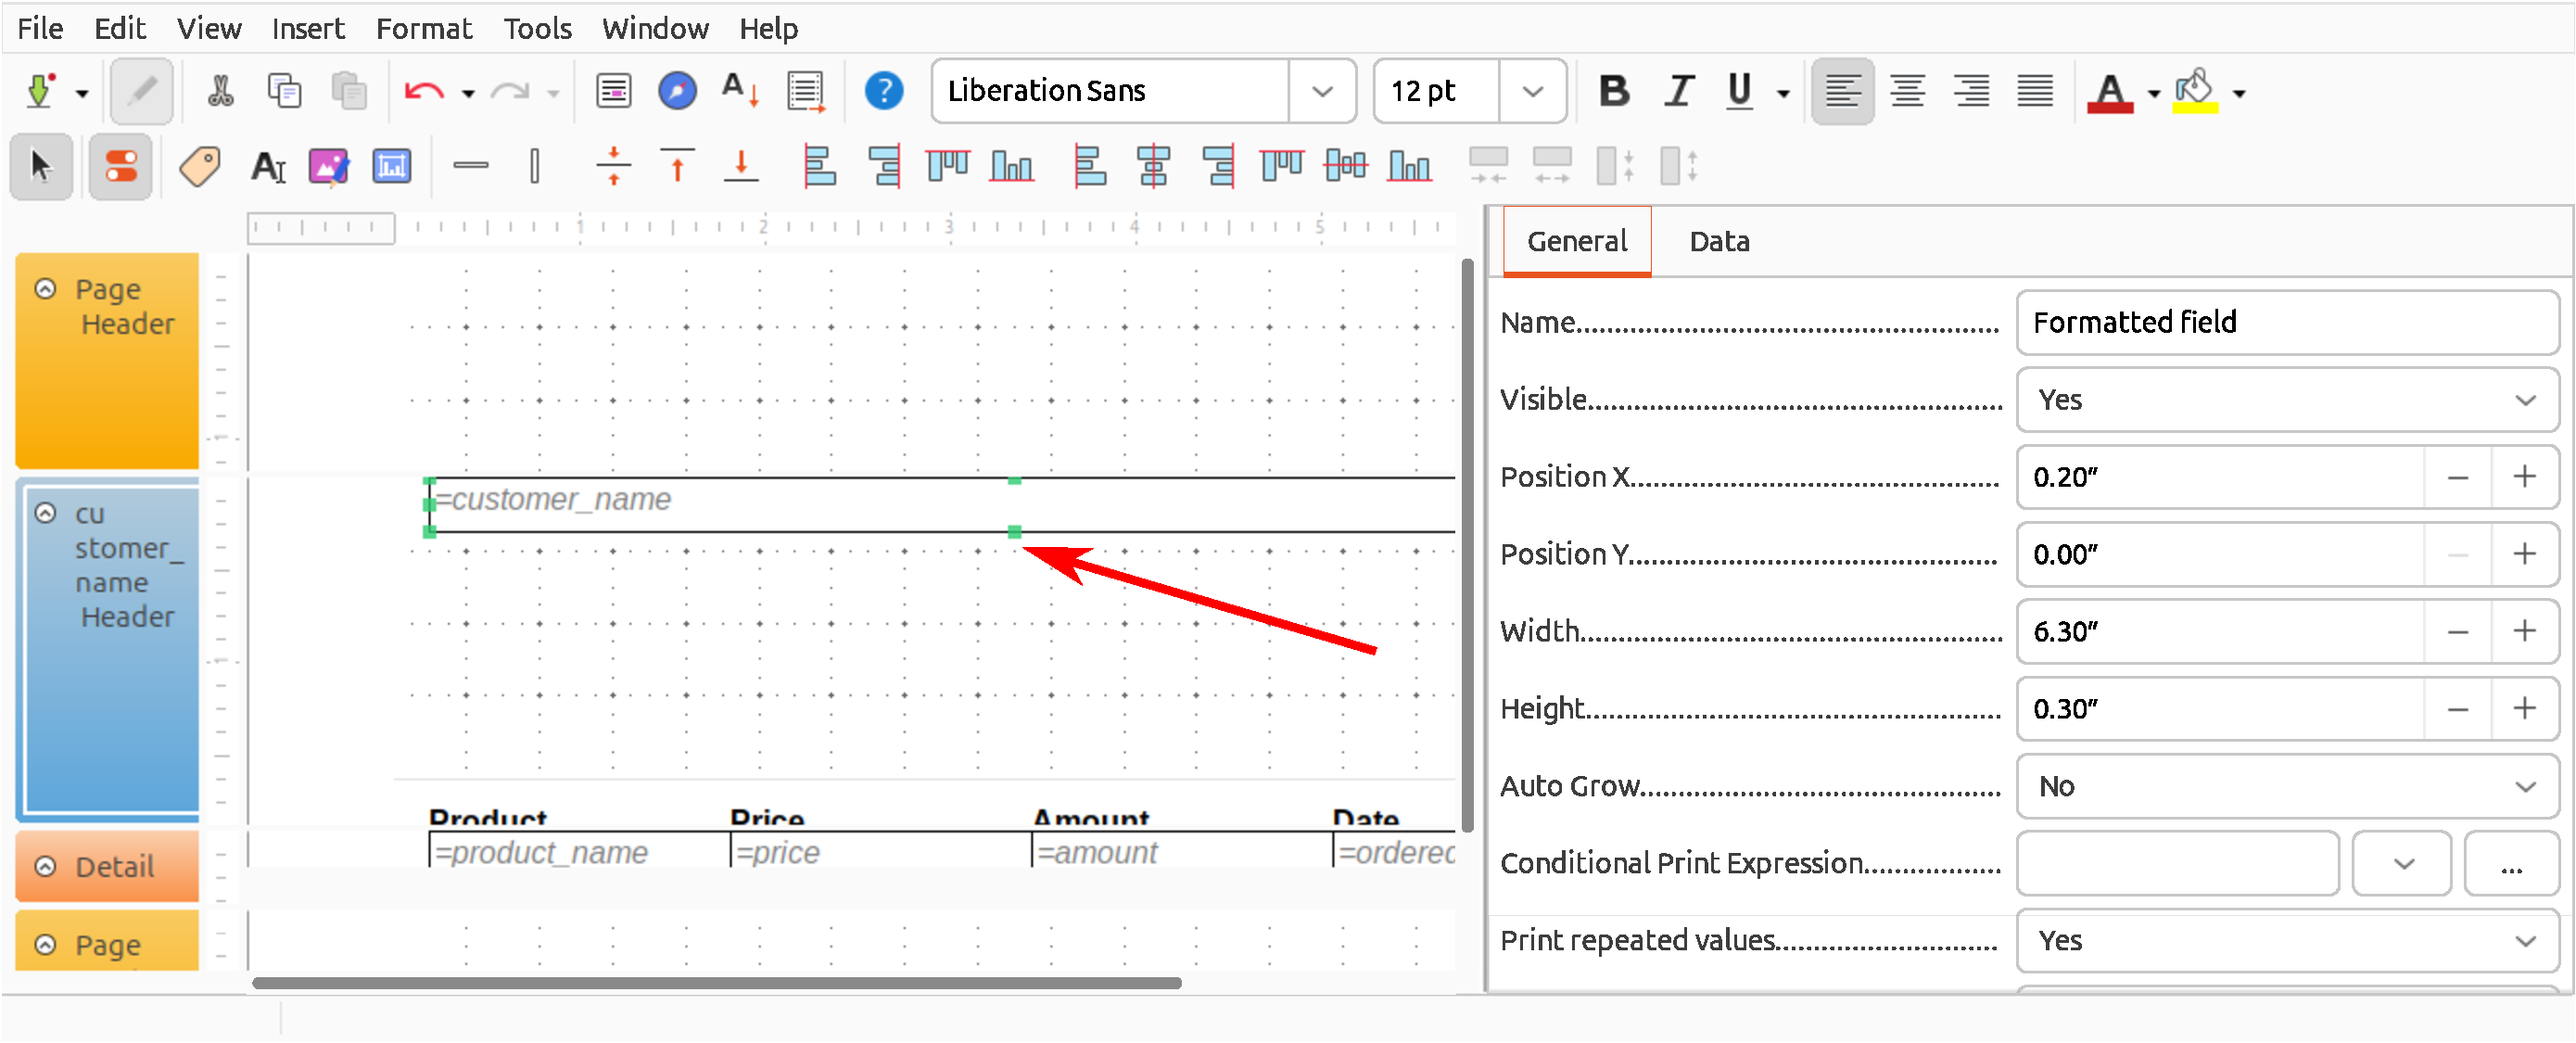
\includegraphics[width=0.49\linewidth]{\currentDir/factoryLibreOfficeBaseReport19customerShrinked}}}%
%
\floatSep%
%
\subfloat[][%
We right-click and drag a selection box around the table header and the horizontal line. %
Then we press the \keys{\arrowkeyup} key to move the header up.%
\label{fig:factoryLibreOfficeBaseReport20headerSelected}%
]{\tightbox{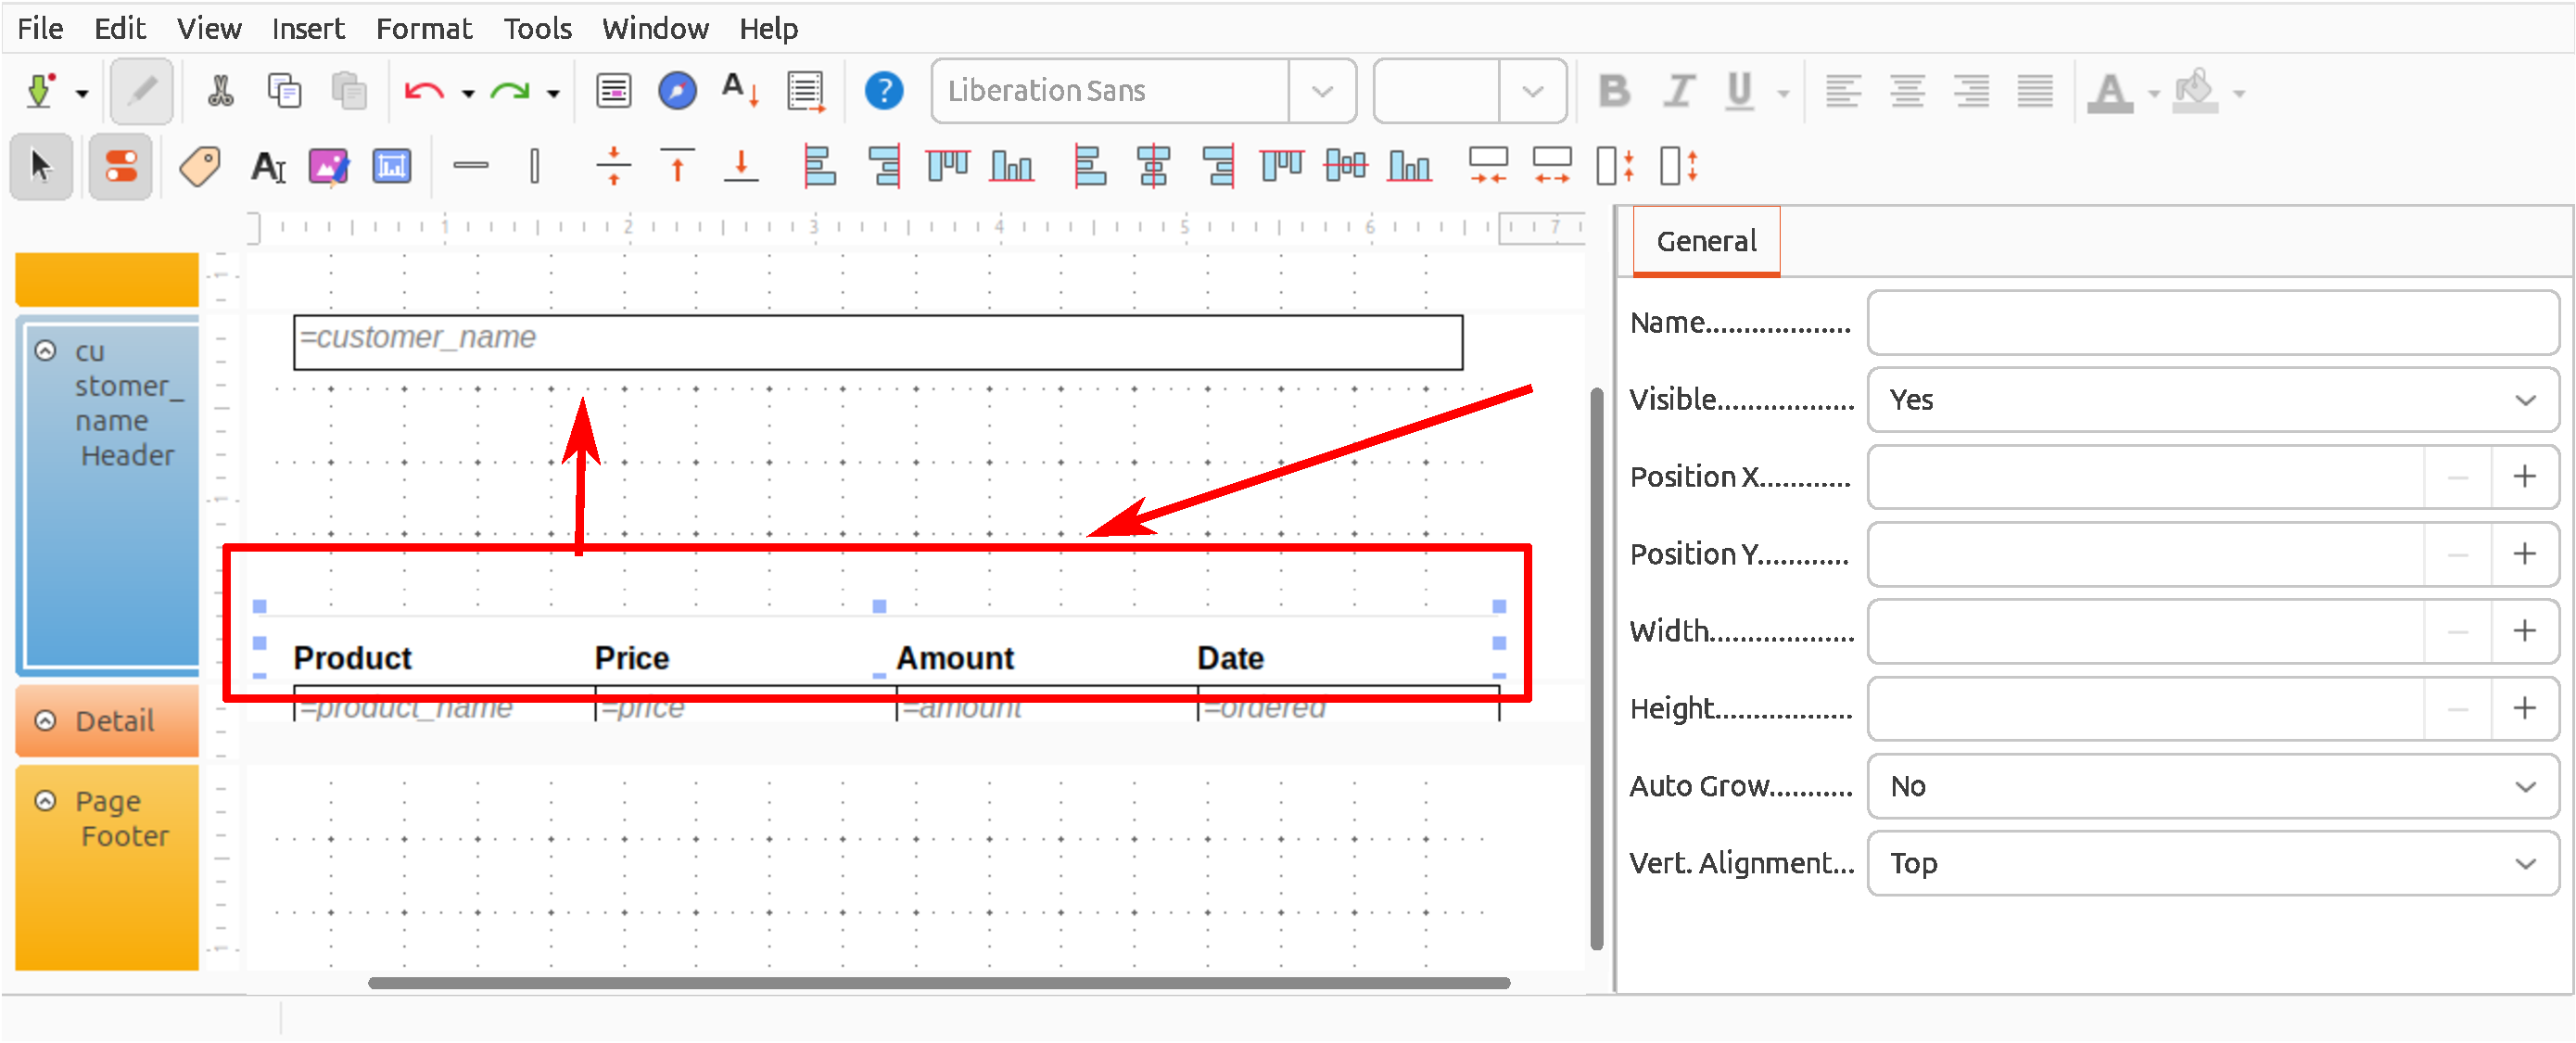
\includegraphics[width=0.49\linewidth]{\currentDir/factoryLibreOfficeBaseReport20headerSelected}}}%
%
\floatRowSep%
%
\subfloat[][%
The header is now moved up.%
\label{fig:factoryLibreOfficeBaseReport21headerMovedUp}%
]{\tightbox{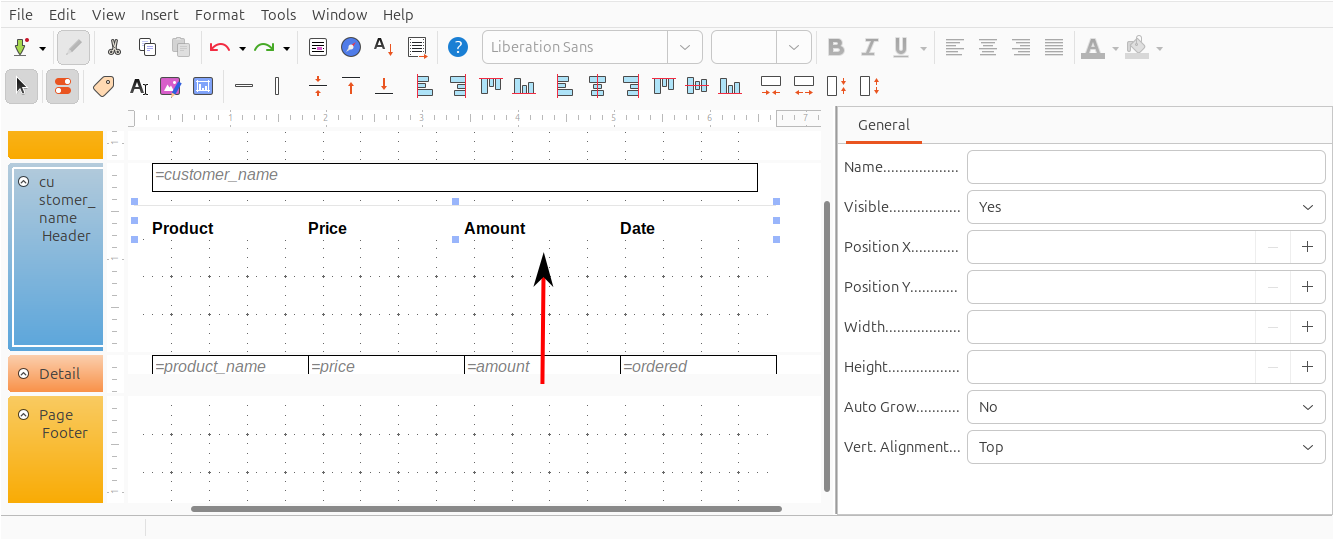
\includegraphics[width=0.49\linewidth]{\currentDir/factoryLibreOfficeBaseReport21headerMovedUp}}}%
%
\floatSep%
%
\subfloat[][%
We now want to make the group header field of the report a bit smaller, so we click on the \inQuotes{customer\_name Header} pane and then into the \menu{Height} property.%
\label{fig:factoryLibreOfficeBaseReport22headerDeselected}%
]{\tightbox{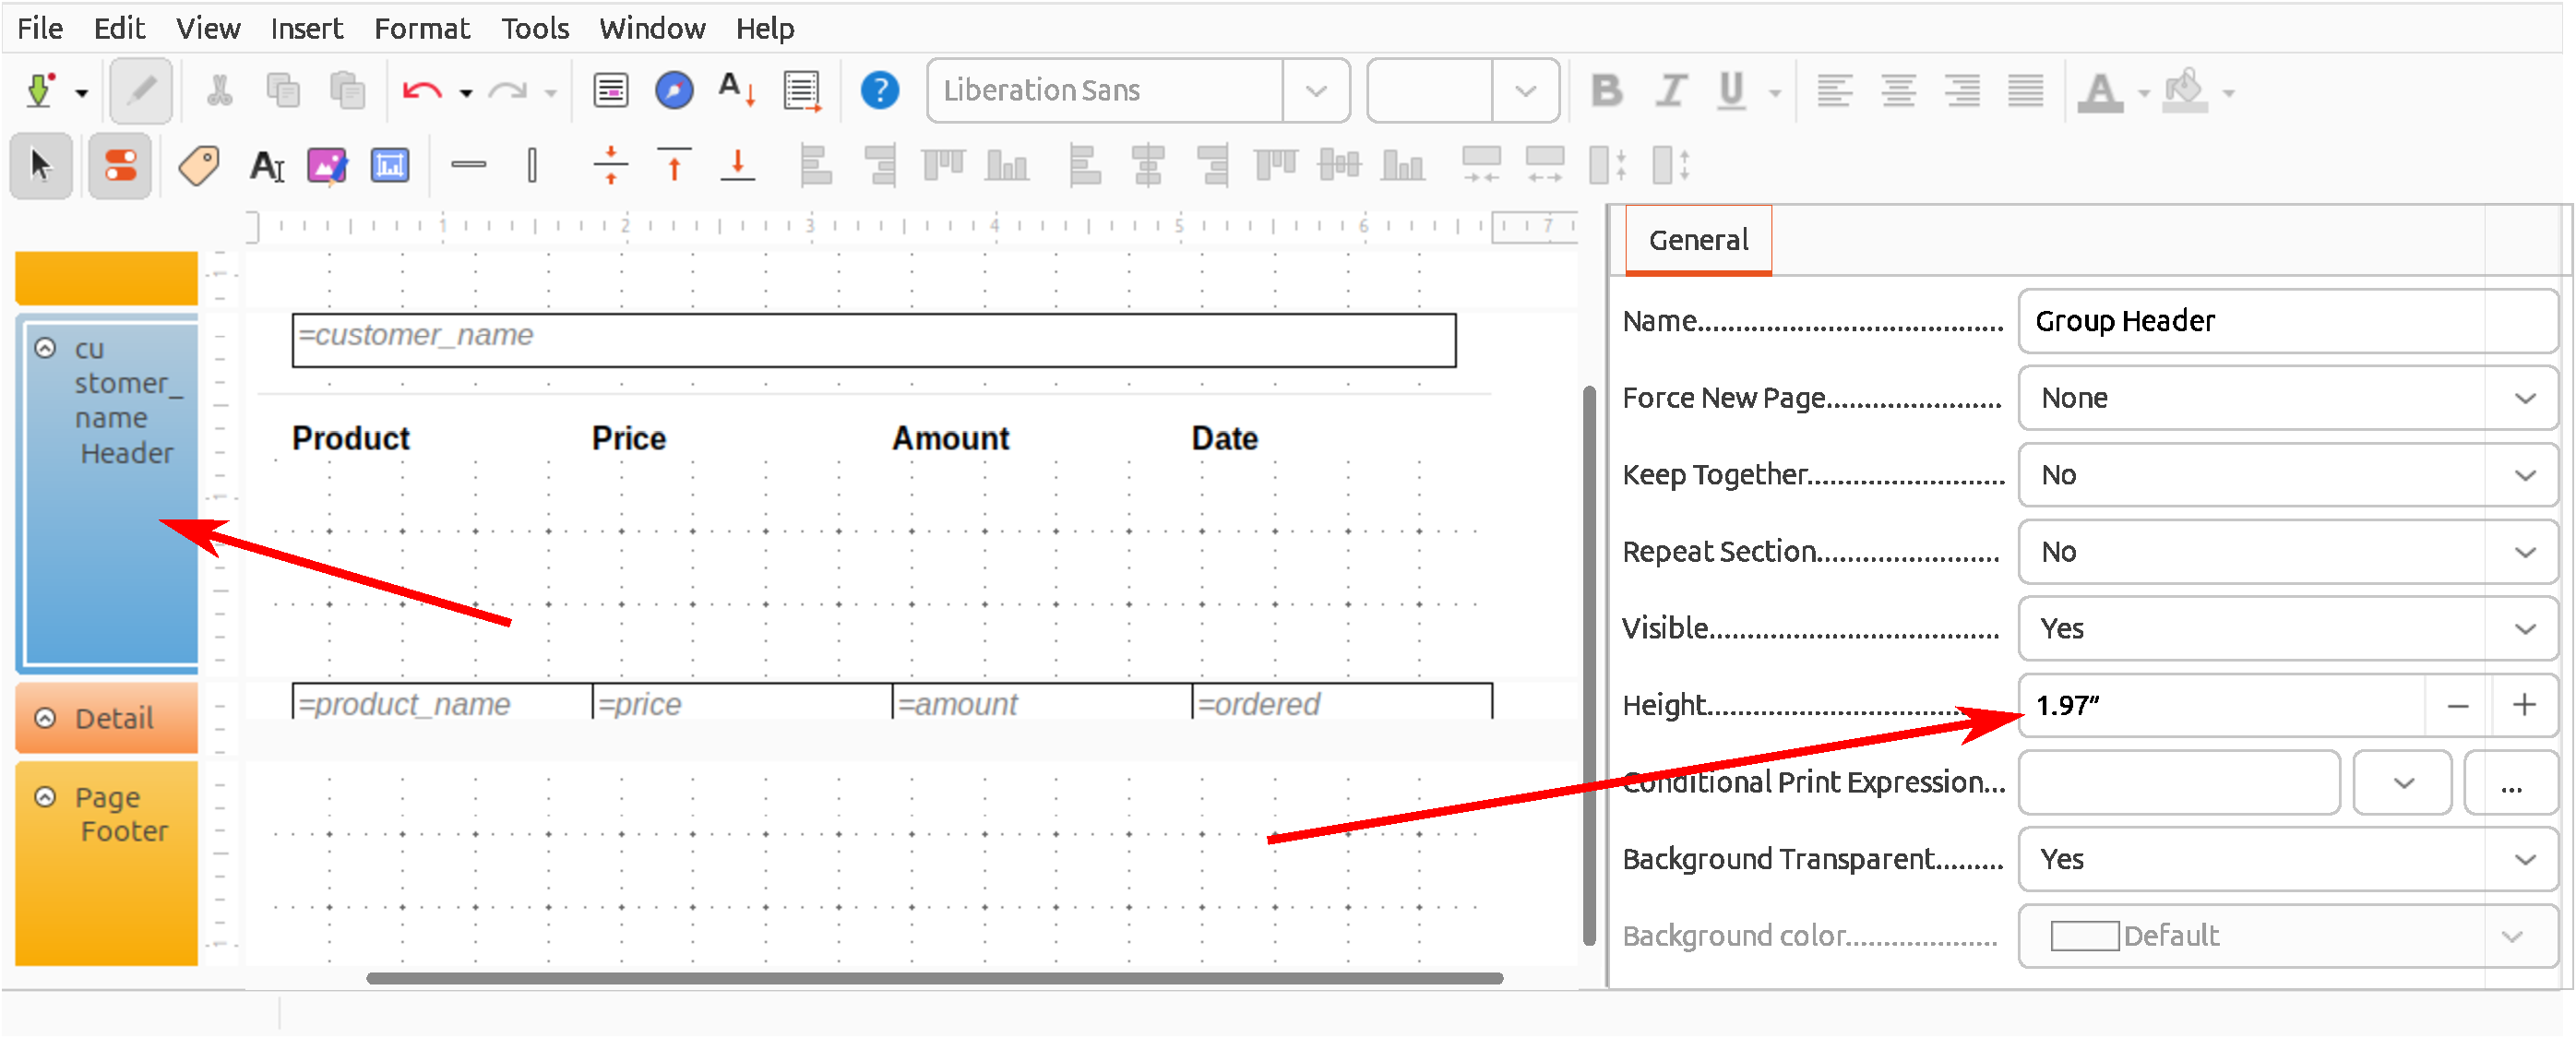
\includegraphics[width=0.49\linewidth]{\currentDir/factoryLibreOfficeBaseReport22headerDeselected}}}%
%
\floatRowSep%
%
\subfloat[][%
We make it nice and small. %
Finally, to create some space between customer groups, we want to move all the header controls down a bit again.%
\label{fig:factoryLibreOfficeBaseReport23headerShrunk}%
]{\tightbox{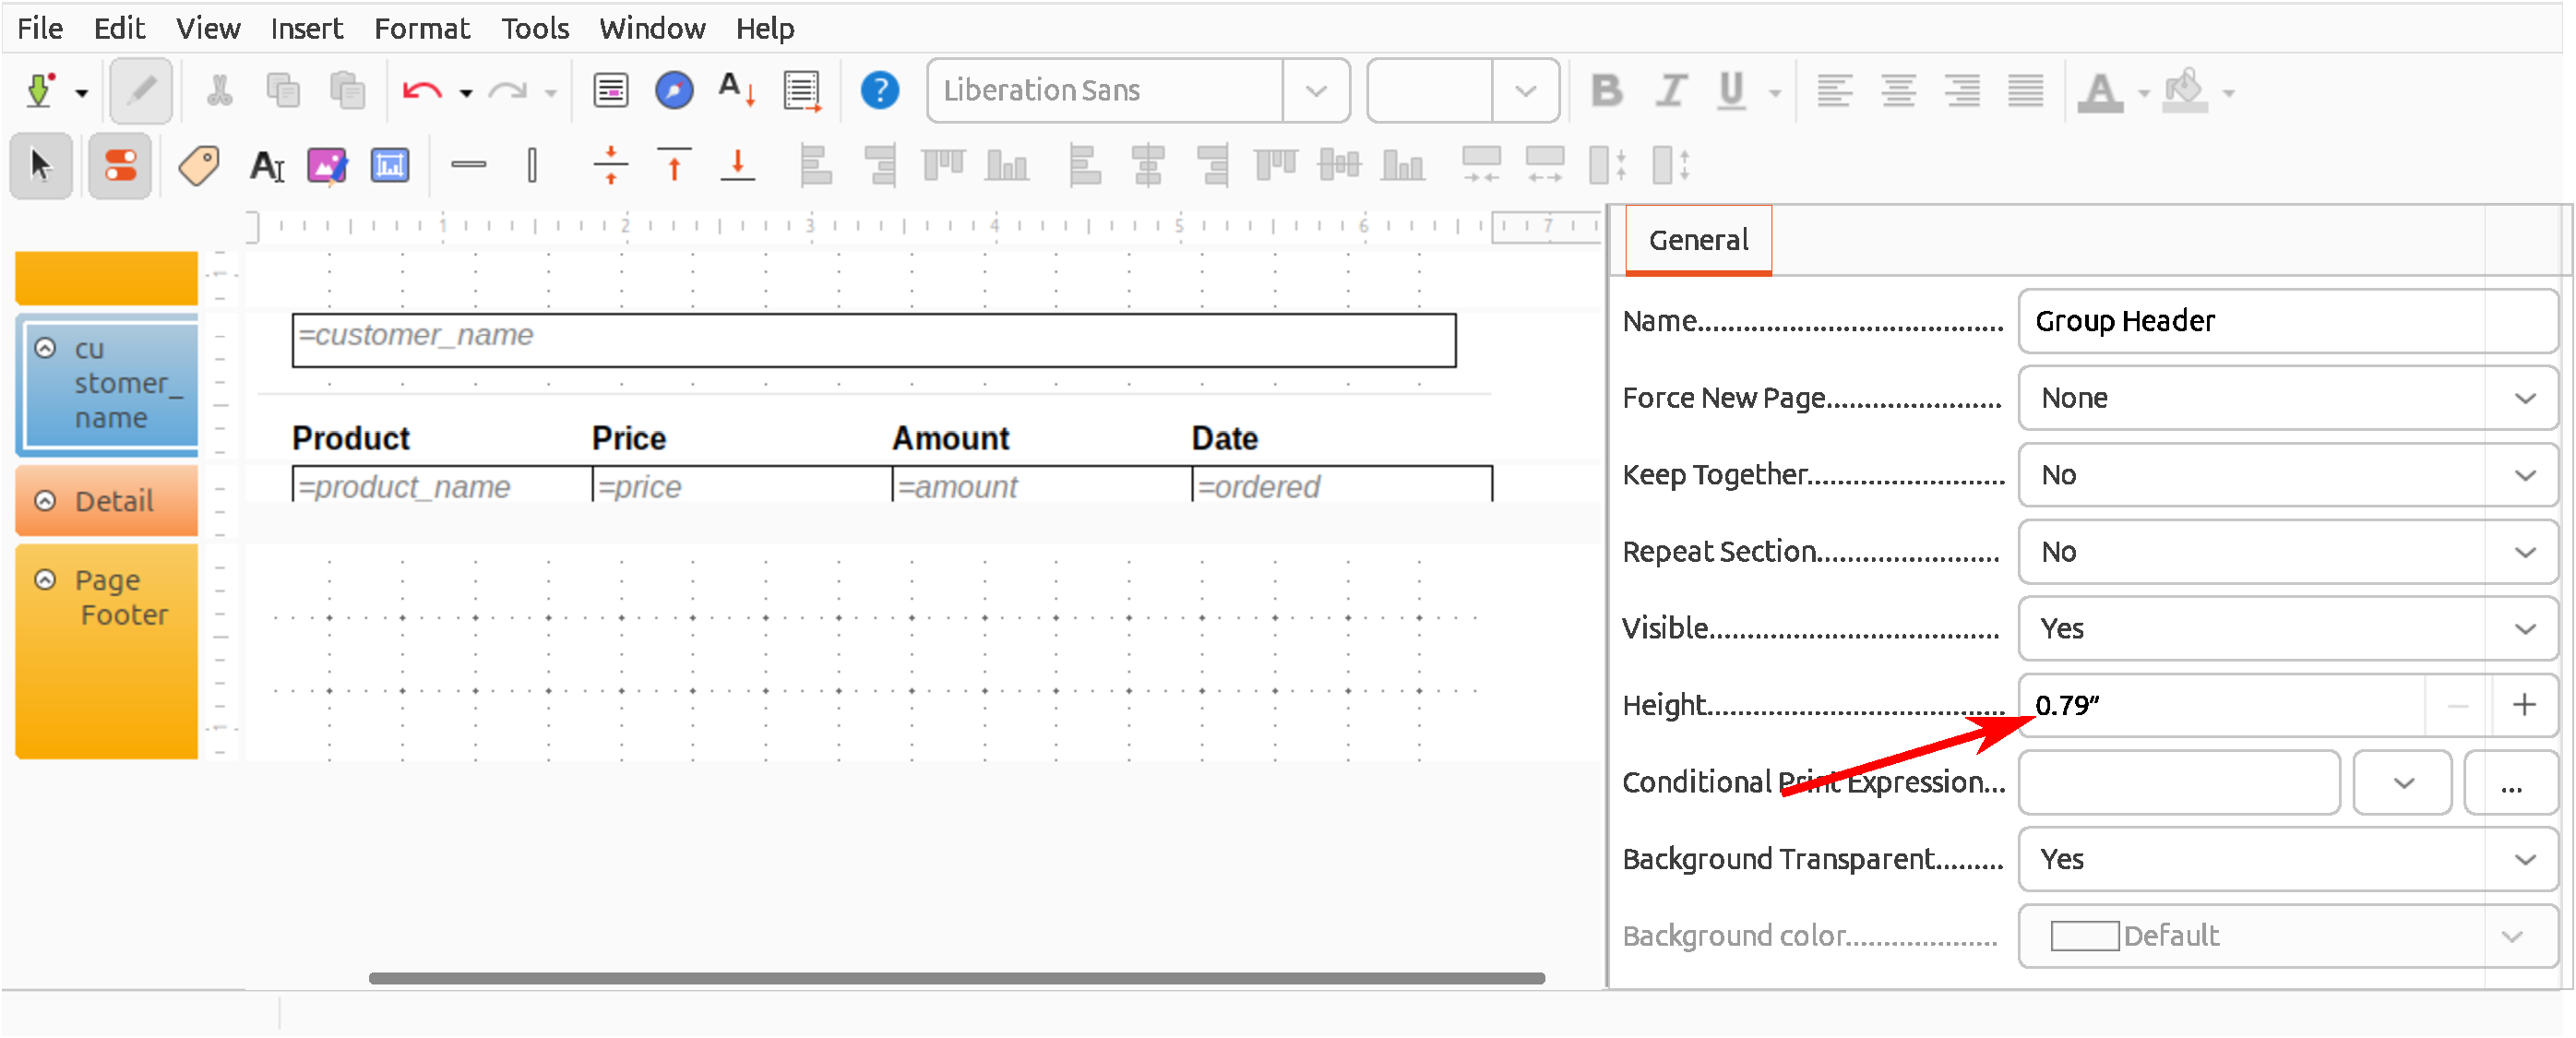
\includegraphics[width=0.49\linewidth]{\currentDir/factoryLibreOfficeBaseReport23headerShrunk}}}%
%
\floatSep%
%
\subfloat[][%
To move them all down, we select them first. %
We right-click into the report and drag a selection box over them.%
\label{fig:factoryLibreOfficeBaseReport24headerSelected}%
]{\tightbox{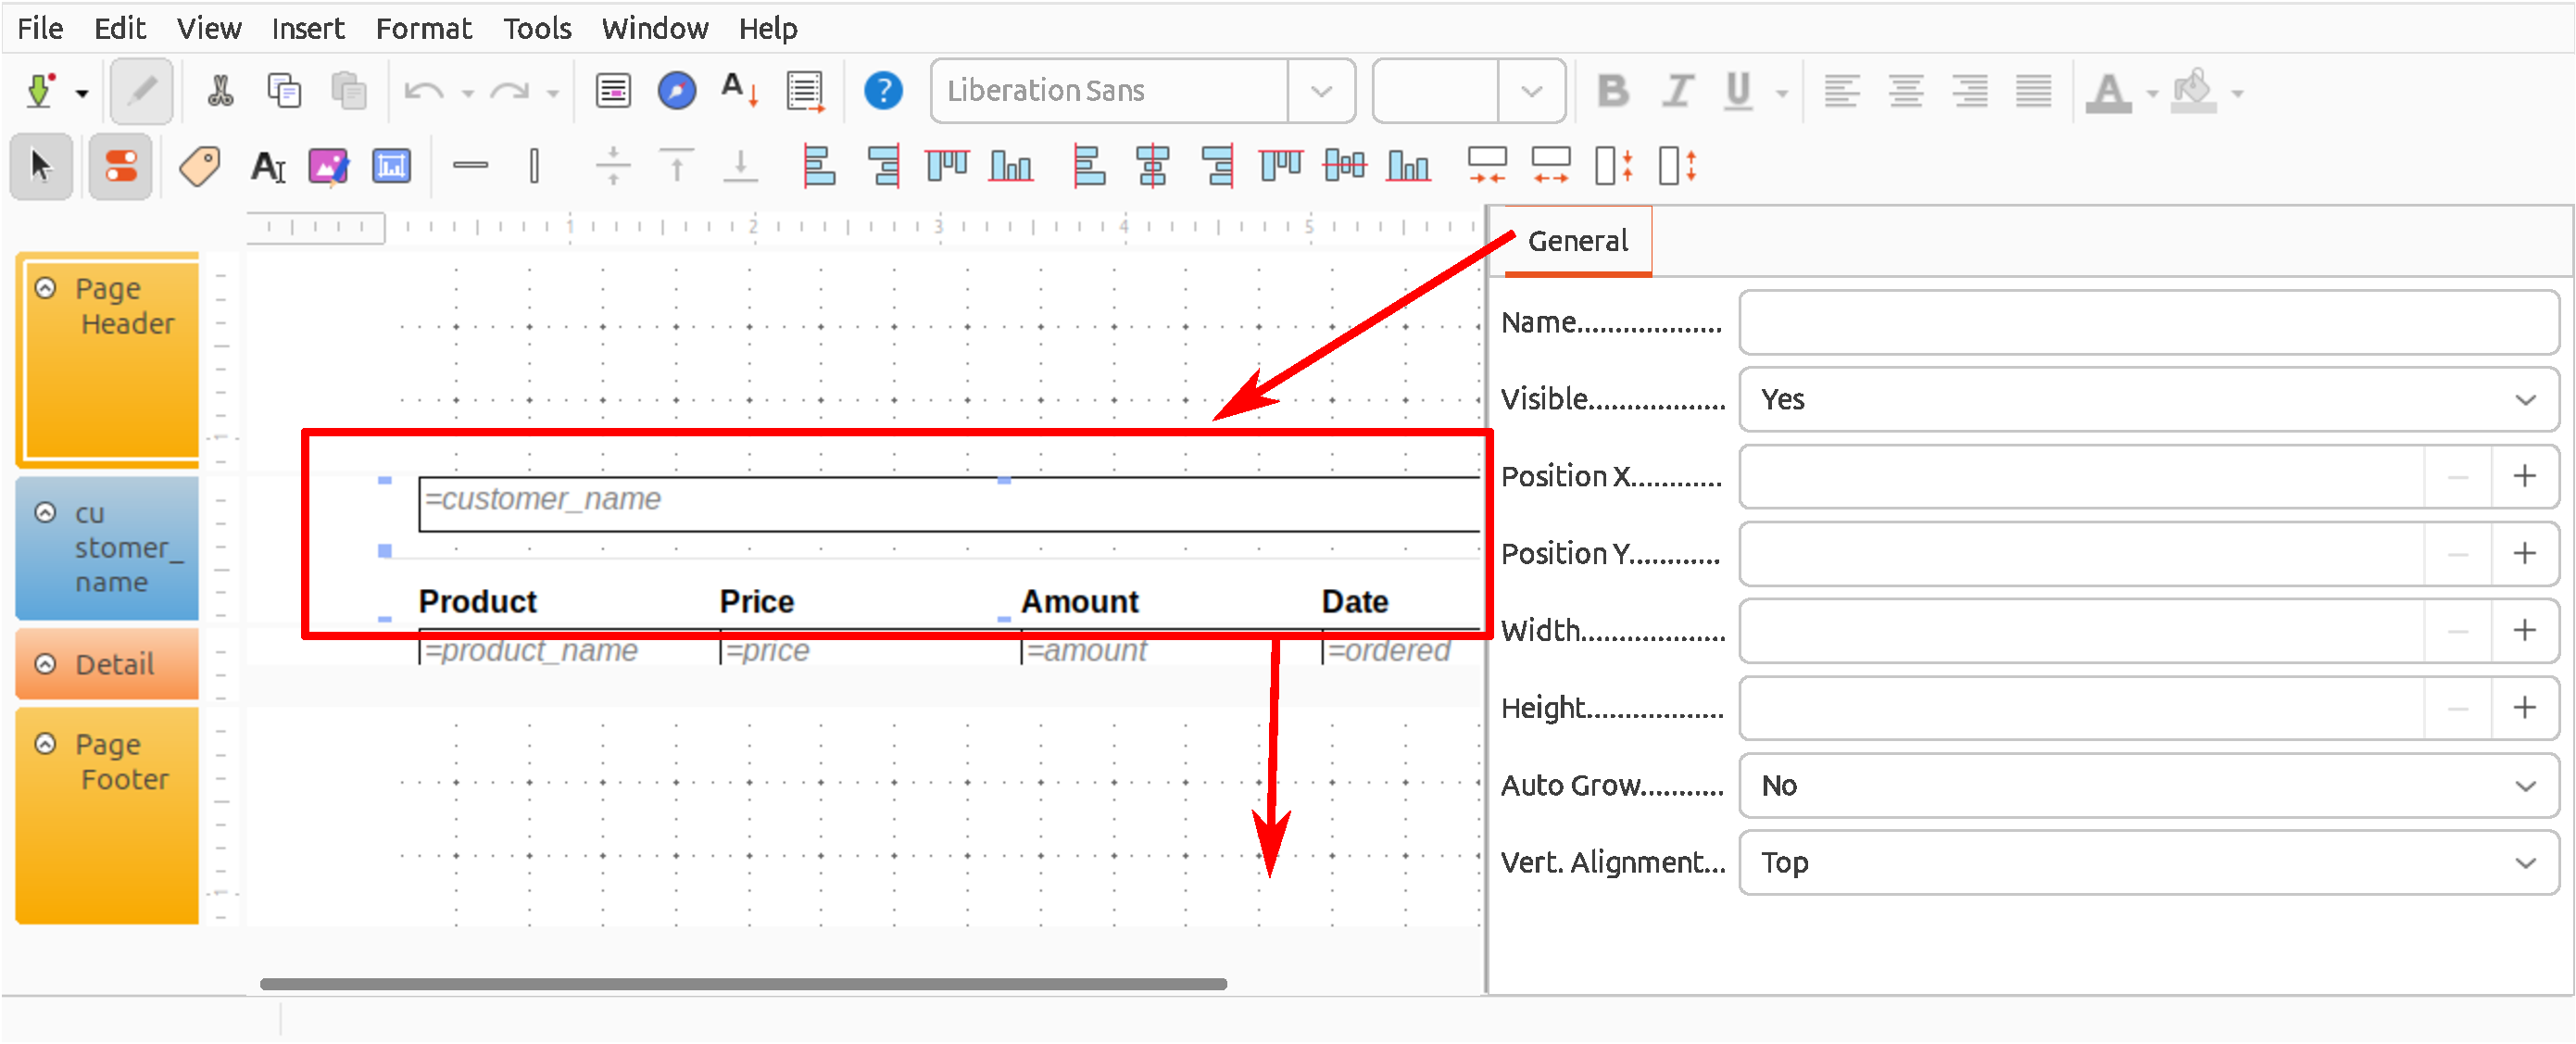
\includegraphics[width=0.49\linewidth]{\currentDir/factoryLibreOfficeBaseReport24headerSelected}}}%
%
\floatRowSep%
%
\subfloat[][%
Then we press the \keys{\arrowkeydown} key a few times. %
We are done and close the report.%
\label{fig:factoryLibreOfficeBaseReport25headerMovedDown}%
]{\tightbox{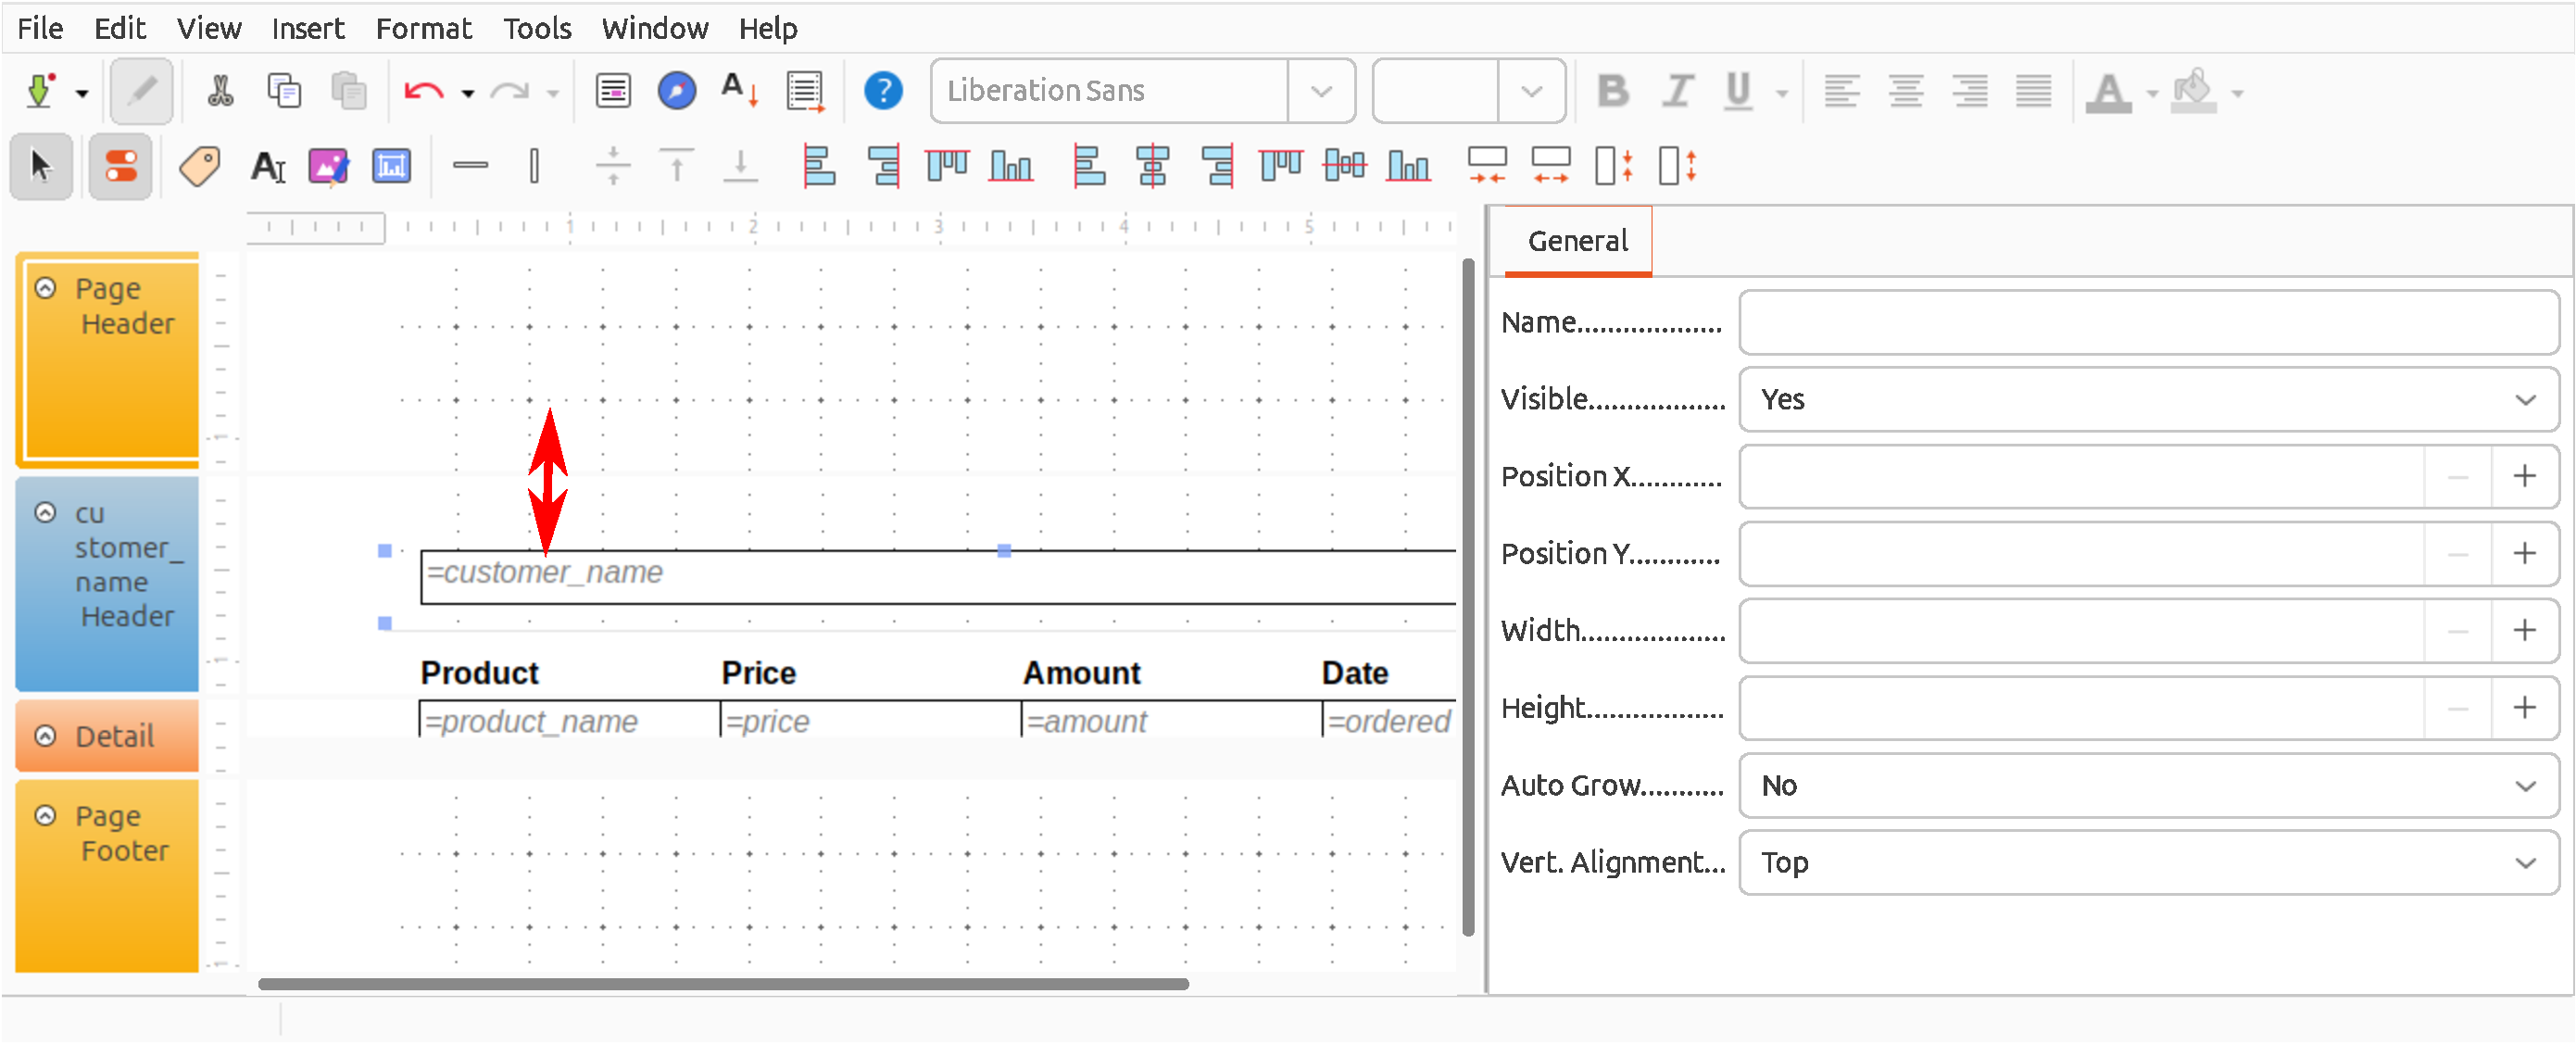
\includegraphics[width=0.49\linewidth]{\currentDir/factoryLibreOfficeBaseReport25headerMovedDown}}}%
%
\floatSep%
%
\subfloat[][%
Upon closing the report, we get asked whether want to save it. %
We click on \menu{save}. %
We save it under the name \textil{sale}.%
\label{fig:factoryLibreOfficeBaseReport26save}%
]{\tightbox{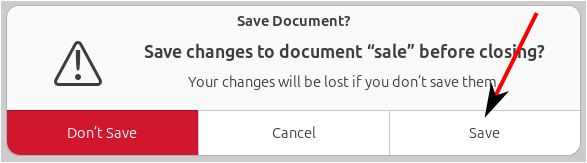
\includegraphics[width=0.49\linewidth]{\currentDir/factoryLibreOfficeBaseReport26save}}}%
%
\caption{Creating and executing \db\ reports in \libreofficeBase\ (Continued).}%
\label{fig:factoryLibreOfficeBaseReportD}%
\end{figure}%
%
%
\begin{figure}%
\ContinuedFloat%
\centering%
%
\subfloat[][%
And it appears under this name in the \menu{Reports} pane. %
We double-click on it. %
\label{fig:factoryLibreOfficeBaseReport27saved}%
]{\tightbox{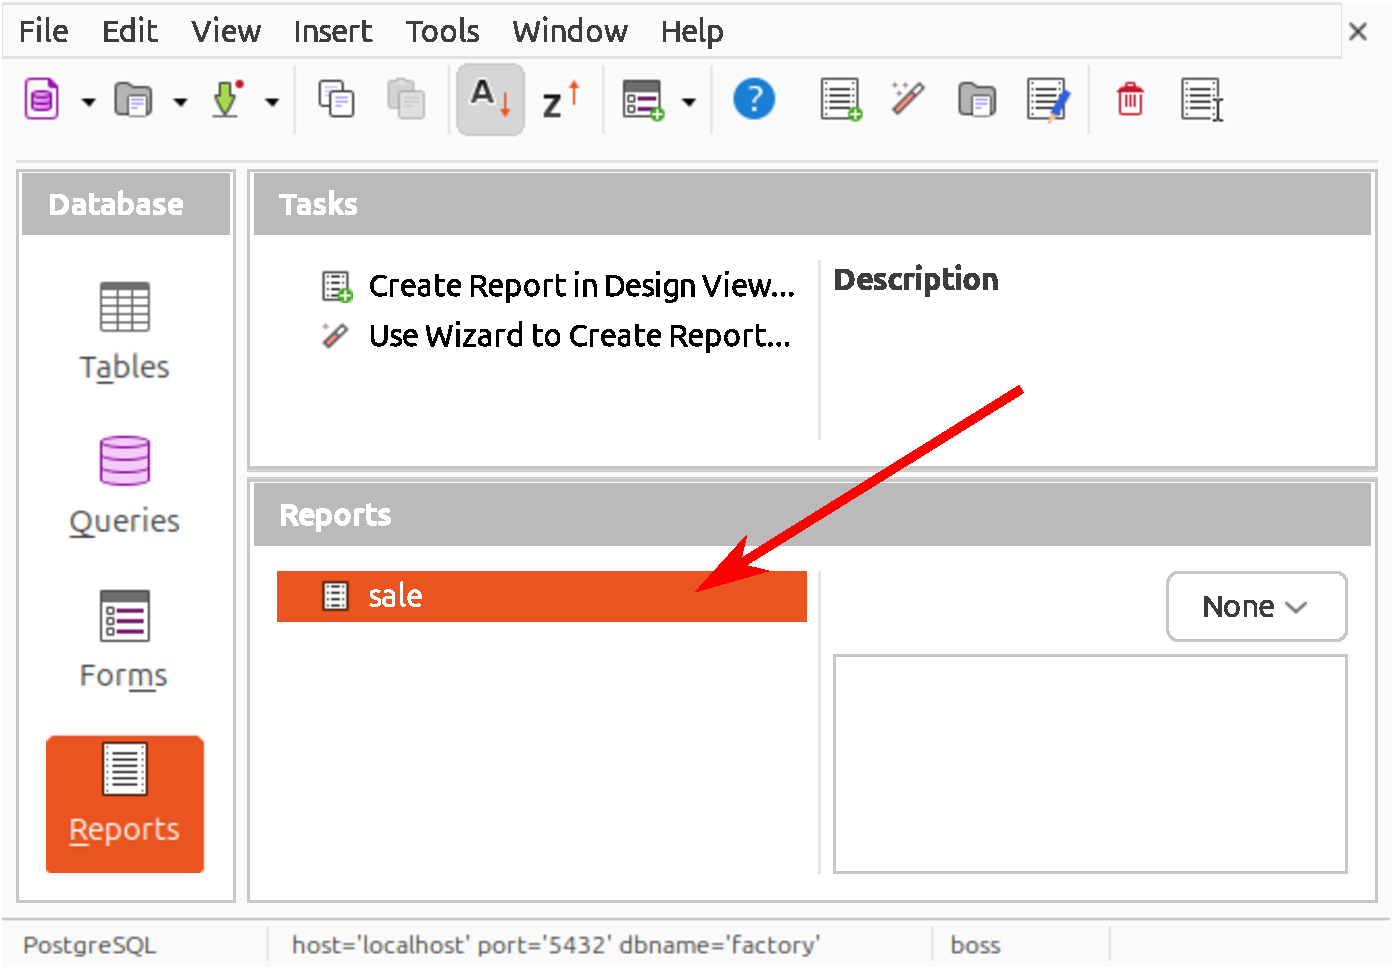
\includegraphics[width=0.49\linewidth]{\currentDir/factoryLibreOfficeBaseReport27saved}}}%
%
\floatSep%
%
\subfloat[][%
A new document opens in \libreoffice\ \softwareStyle{Write}. %
It contains all the data in a very nicely formatted fashion. %
We can even export it to PDF by clicking the PDF symbol.%
\label{fig:factoryLibreOfficeBaseReport28executed}%
]{\tightbox{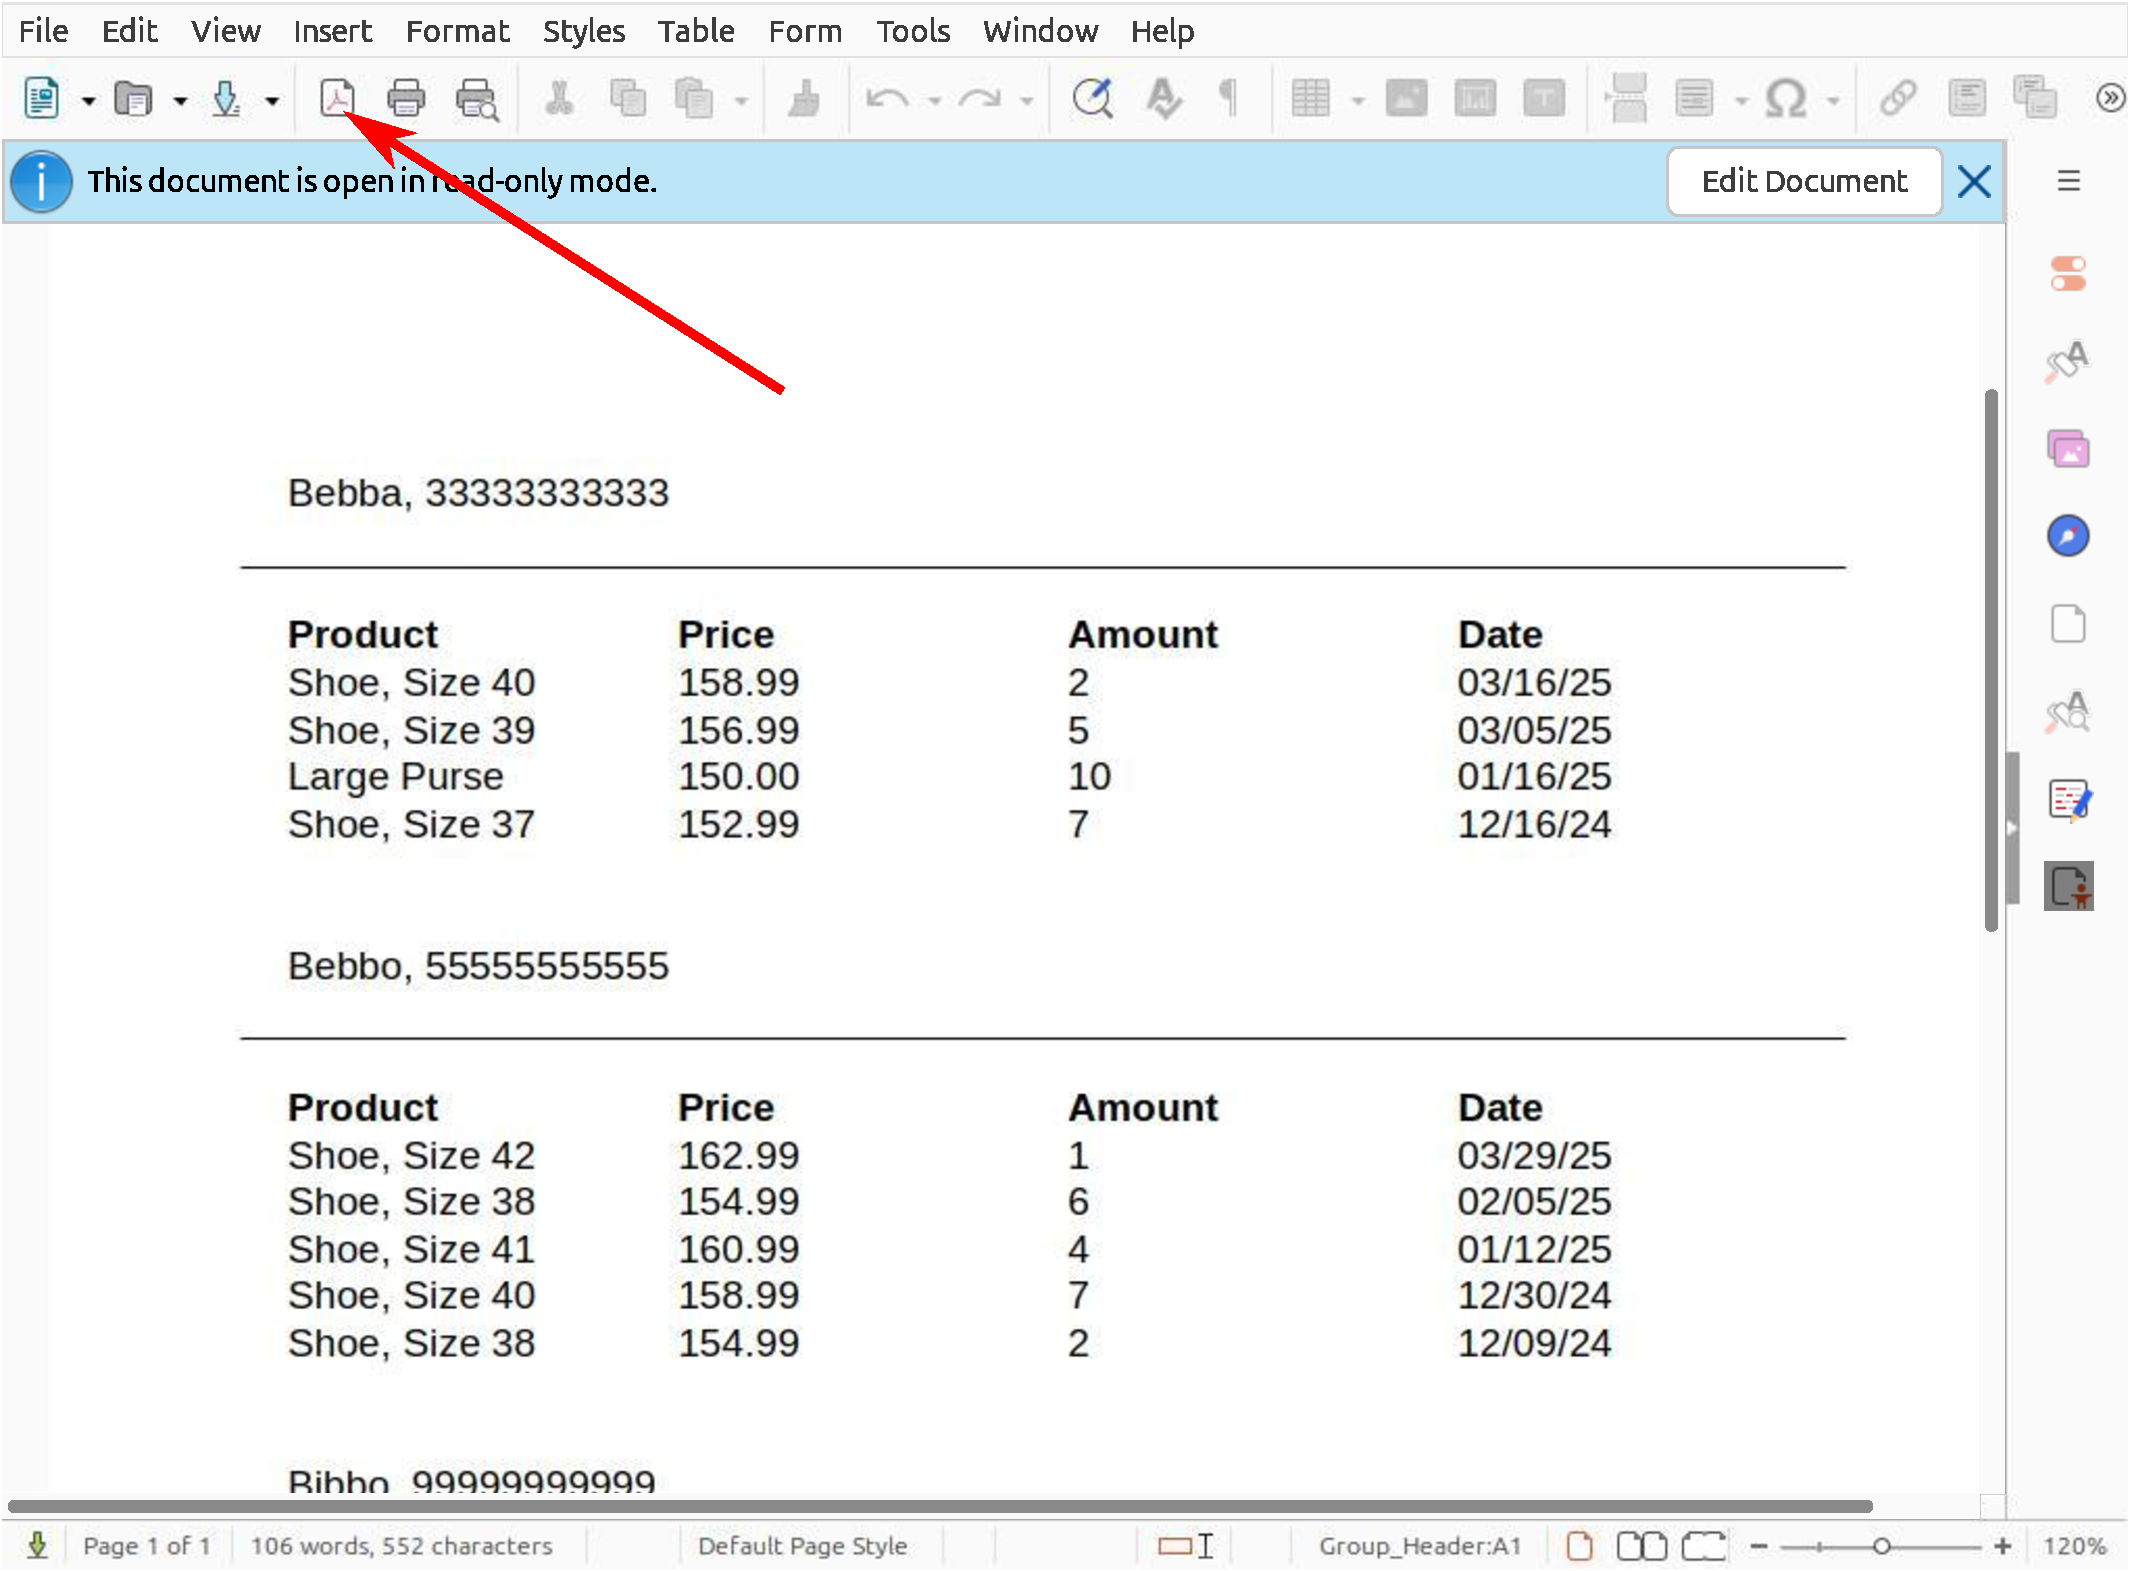
\includegraphics[width=0.49\linewidth]{\currentDir/factoryLibreOfficeBaseReport28executed}}}%
%
\floatRowSep%
%
\subfloat[][%
The exported PDF document.%
\label{fig:factoryLibreOfficeBaseReport29report}%
]{\tightbox{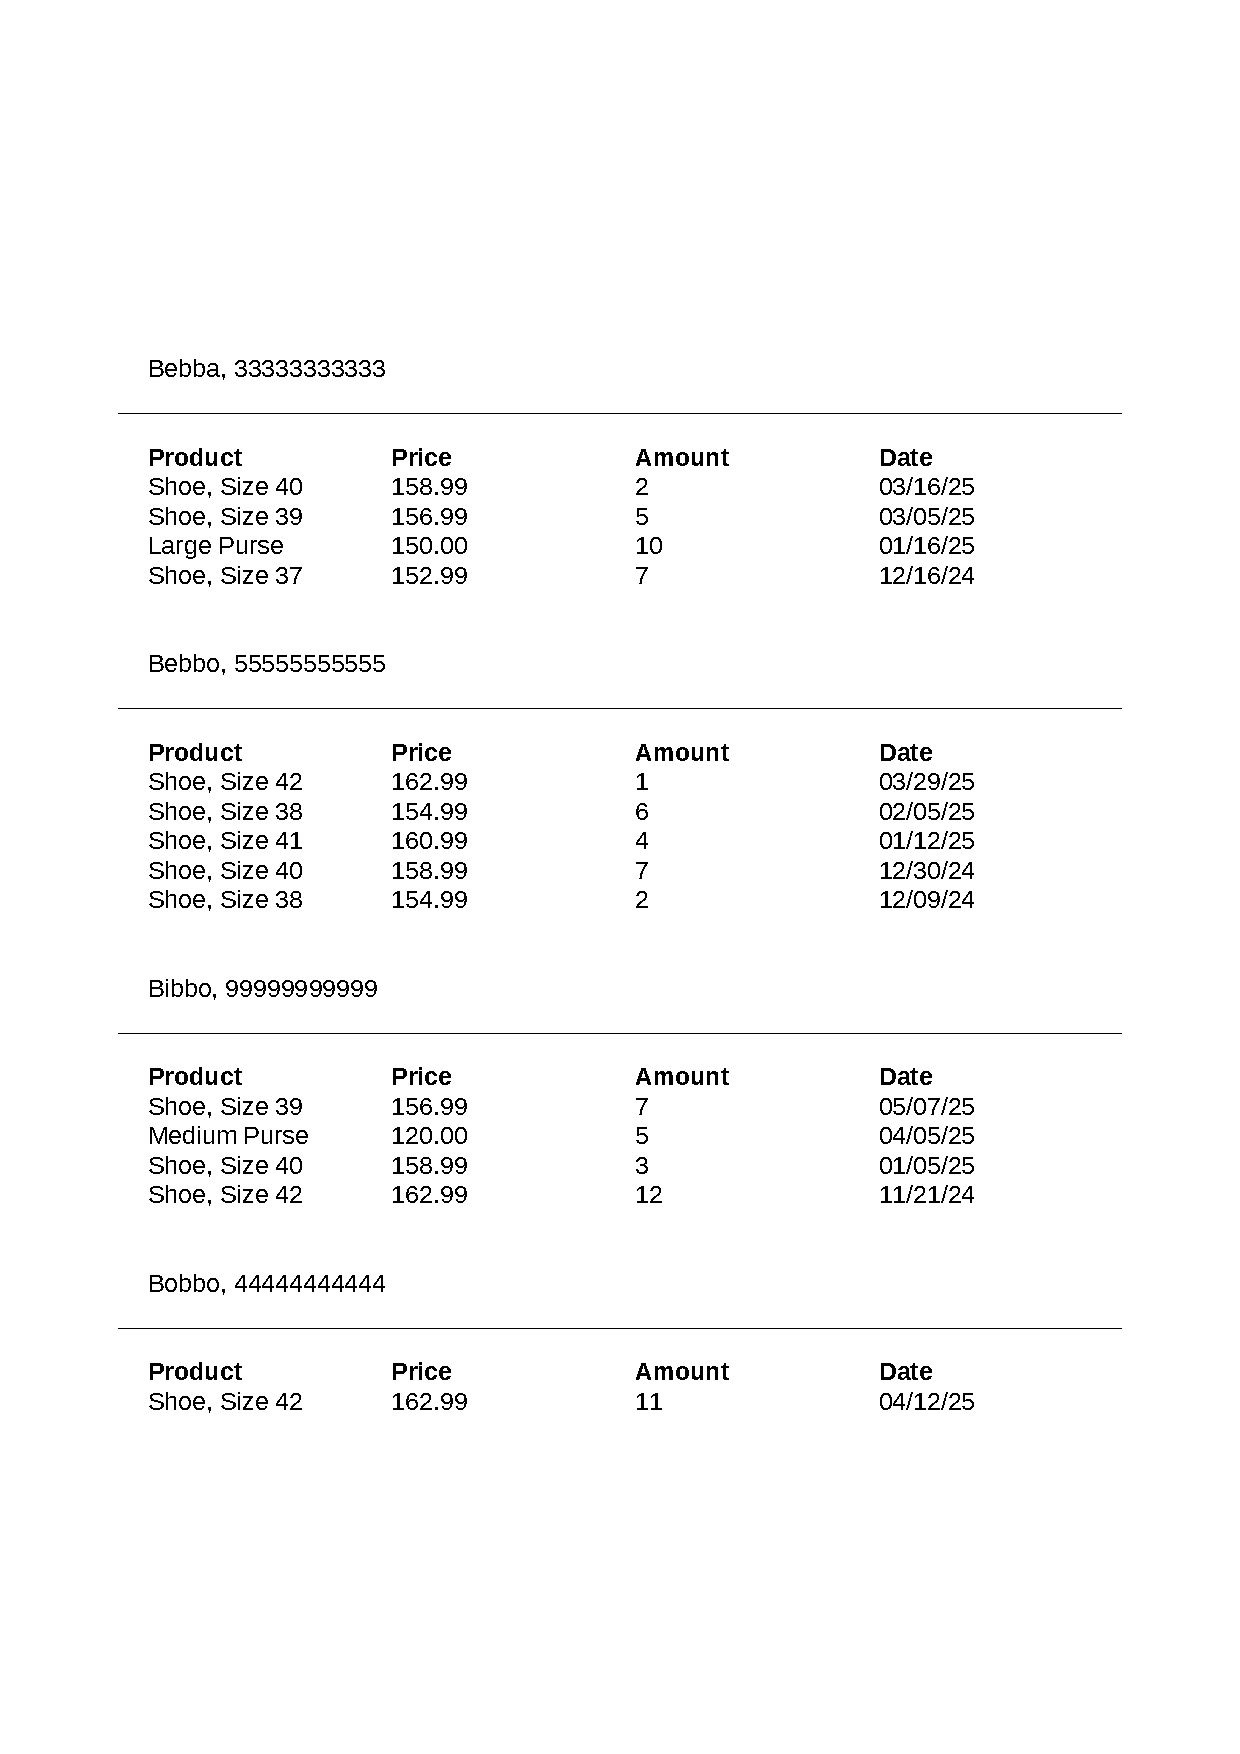
\includegraphics[width=0.49\linewidth]{\currentDir/factoryLibreOfficeBaseReport29report}}}%
%
\caption{Creating and executing \db\ reports in \libreofficeBase\ (Continued).}%
\label{fig:factoryLibreOfficeBaseReportE}%
\end{figure}%
%
\FloatBarrier%
\endhsection%
%
